\chapter{Méthodes}

Nous avons utilisé la base de données présentée dans la partie~\ref{lab:bdd} pour évaluer les performances des techniques de correction du mouvement respiratoire présentées dans le chapitre \ref{lab:corrMvt}. 

Les techniques de correction du mouvement implémentées sont les suivantes :

\begin{enumerate}
 \item Correction pendant la reconstruction par modification de la matrice système (voir section \ref{lab:corrMatSyst}). Elle sera désignée par l'acronyme \emph{TE-MS} (Transformation \'Elastique de la Matrice Système)
 \item Correction post-reconstruction par recalage des images prises à différents instants du cycle (voir section \ref{lab:corrPostRecon}). Elle sera désignée par l'acronyme \emph{TE-IM} (Transformation \'Elastique des IMages reconstruites) 
\end{enumerate}

Les images TEP corrigées à l'aide de ces deux méthodes sont comparées dans cette partie avec les images non corrigées et des images statiques (qui représentent une correction parfaite). Leurs acronymes sont respectivement \emph{NoCorr} et \emph{Statique}.

L'objectif est d'évaluer les performances des techniques de correction du mouvement sur la détection des lésions de faible contraste et faible diamètre. Pour cela, les performances d'un système de détection automatique seront mesurées à l'aide des courbes F-ROC.

Ce chapitre va tout d'abord présenter la démarche réalisée pour sélectionner les paramètres de reconstruction des images, puis la méthode d'estimation du mouvement utilisée. 

La suite de ce chapitre présente les caractéristiques principales du système d'aide à la détection (CAD) que nous avons proposé (voir chapitre \ref{lab:chapCAD}), l'étape d'optimisation des paramètres de ce CAD que nous avons utilisé, puis la méthode que nous avons développée pour mesurer les performances de détection.

%%%%%%%%%%%%% EXTRAITE DE LA PARTIE PRECEDENTE



%%%%CASER DESCRIPTION RECONSTRUCTION
%Les images sont reconstruites avec des voxels de 4mm dans les trois dimensions, ce qui correspond à la résolution de l'imageur TEP~\cite{surti2004imaging}. Les reconstructions sont réalisées à l'aide de l'algorithme OPL-EM avec 8 itérations et 5 sous-ensembles sans régularisation, sauf pour l'estimation de mouvement où seulement 3 itérations avec 5 sous-ensembles sont réalisées, avec une régularisation de 6 mm à chaque itération. 
%%%%%

\section{Reconstruction des images}

Nous avons utilisé le logiciel de reconstruction fourni par le laboratoire LaTIM dans le cadre d'un partenariat, créé et utilisé par Frédéric Lamare pour ses travaux sur la correction du mouvement respiratoire~\cite{lamare2007list}.

Ce logiciel est capable de reconstruire les images acquises en données séquentielles à l'aide de l'algorithme OPL-EM décrit en \ref{lab:OPLEM}. La reconstruction permet de prendre en compte la correction de l'atténuation, mais ne permet pas la correction des coïncidences aléatoires et des coïncidences diffusées. Nous avons donc choisi de simplifier le problème en supposant une correction parfaite de ces deux effets. Pour cela, nous n'avons pas inclus les photons diffusés ou les coïncidences aléatoires dans les données séquentielles. 

L'algorithme utilisé peut intégrer les corrections de mouvement à partir d'une estimation du champ de déplacement qui doit être calculé séparément. La qualité de ce champ conditionne la qualité de la correction. De plus, OPL-EM nécessite de choisir le nombre de sous-ensembles d'itération. Cette section présente l'étude réalisée pour fixer ces différents paramètres.

\subsection{Paramètres de reconstruction}
\label{lab:paramRecon}

Lors de l'utilisation des méthodes itératives, il faut définir le nombre d'itérations à appliquer lors de la reconstruction. La figure~\ref{fig:evolRecon} présente des reconstructions  réalisées avec différentes valeurs du nombre d'itérations. L'algorithme OPL-EM utilisé pour réaliser les reconstructions emploie la technique des sous-ensembles pour accélérer la reconstruction.

Le nombre d'itérations totale (nombre d'itération $\times$ Nombre de sous-ensemble) va déterminer la qualité du résultat. Nous avons choisi de travailler avec 5 sous-ensembles et de faire varier le nombre d'itérations de 1 à 7, ce qui correspond à une évaluation de 5 à 35 itérations totales.

\begin{figure}
\centering
\begin{tabular}{c c c c}
 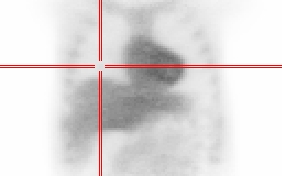
\includegraphics[width=3cm]{images/ite1} & 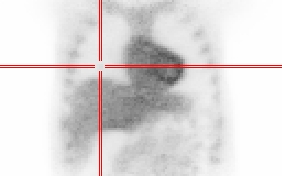
\includegraphics[width=3cm]{images/ite3} & 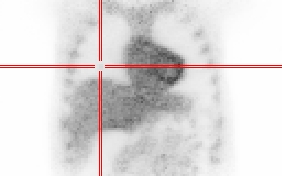
\includegraphics[width=3cm]{images/ite5} & 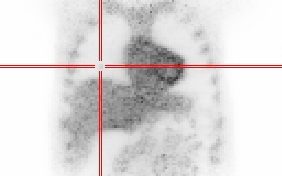
\includegraphics[width=3cm]{images/ite7} \\
Itération 1  & Itération 3 & Itération 5 & Itération 7 \\
\hline
 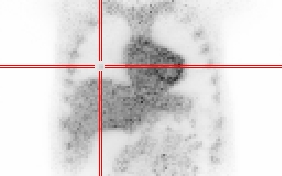
\includegraphics[width=3cm]{images/ite9} & 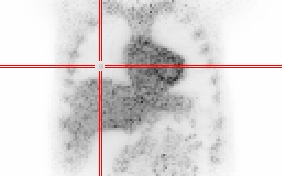
\includegraphics[width=3cm]{images/ite11} & 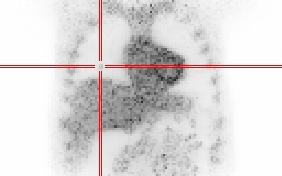
\includegraphics[width=3cm]{images/ite13} &  \\
Itération 9  & Itération 11 & Itération 13 &\\
\end{tabular}

\caption[Illustration de l'évolution des lésions en fonction du nombre d'itérations]{Illustration de l'évolution des images en fonction du nombre d'itérations utilisées pour la reconstruction. Une lésion est présente au centre de la croix rouge.}
\label{fig:evolRecon}
\end{figure}

L'optimisation du nombre totale d'itérations est réalisée en maximisant le rapport contraste sur bruit~\cite{takahara2004diffusion} (CSB) des lésions, défini comme suit :

\begin{equation}
 CSB = \frac{µ_{signal} - µ_{fond}}{\sqrt{\sigma_0}}
\end{equation}

Où $µ_{signal}$ et $µ_{fond}$ représentent, respectivement, l'activité moyenne d'une zone d'intérêt de taille 3$\times$3$\times$3 voxels centrée sur une lésion, et l'activité moyenne d'une zone saine. Cette zone saine correspond à un volume de 200 voxels dans le poumon et de 64 voxels dans le foie. $\sigma_0$ représente la variance du bruit. Dans notre cas, cette variance est évaluée sur la zone saine définie précédemment. Appliquée aux lésions, cette métrique a l'avantage de permettre une représentation rapide de l'évolution du contraste entre la lésion et le fond, tout en pénalisant le bruit.

L'évaluation du rapport contraste sur bruit est réalisée sur une acquisition statique d'un modèle de patient contenant 12 lésions (6 dans le foie et 6 dans le poumon), de diamètre et de contraste échantillonnés à partir des valeurs calibrées dans la table \ref{tab:contrastePoumonFoieRecap} présentée à la page \pageref{tab:contrastePoumonFoieRecap}.

Les résultats sont présentés dans la figure \ref{fig:CNRFoie} pour le foie et \ref{fig:CNRPoumon} pour le poumon.

\begin{figure}
\centering
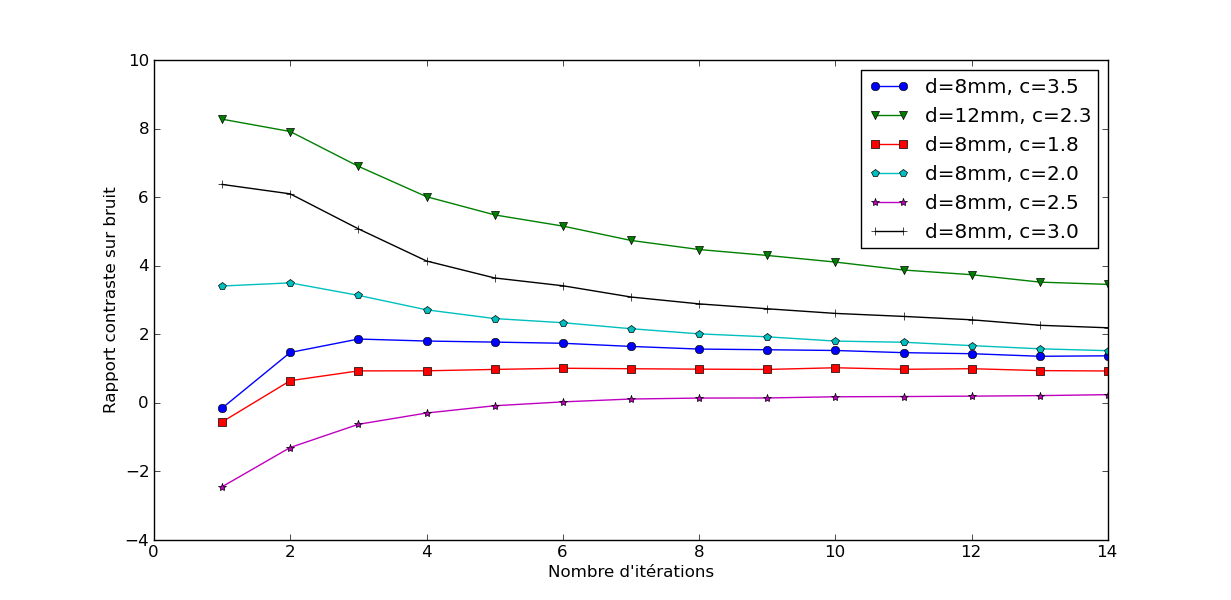
\includegraphics[width=17cm]{images/CNRFoie}
\caption[Evaluation du rapport contraste sur bruit des lésions du foie en fonction du nombre d'itérations]{Evaluation du rapport "contraste sur bruit" des lésions du foie en fonction du nombre d'itérations : sont indiqués, pour chaque lésion, le niveau de contraste réel ainsi que le diamètre de la lésion}
\label{fig:CNRFoie}
\end{figure}


\begin{figure}
\centering
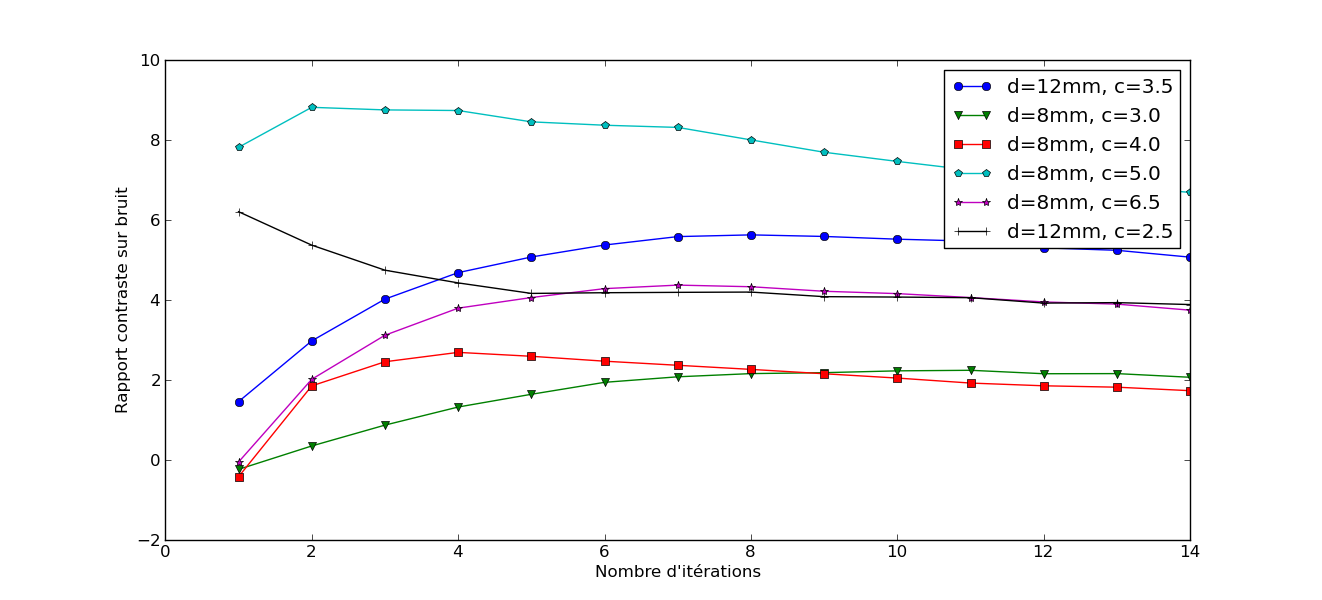
\includegraphics[width=17cm]{images/CNRPoumon}
\caption[Evaluation du rapport "contraste sur bruit" des lésions du poumon en fonction du nombre d'itérations]{Evaluation du rapport Contraste sur bruit des lésions du poumon en fonction du nombre d'itérations : sont indiqués, pour chaque lésion, le niveau de contraste réel ainsi que le diamètre de la lésion}
\label{fig:CNRPoumon}
\end{figure}

La première observation est que certaines courbes sont strictement descendantes, surtout dans le foie. Cela s'explique par le fait que le niveau de bruit augmente beaucoup plus rapidement que la différence d'activité entre le signal et le fond. Cependant, les lésions concernées ont toutes un contraste très élevé, ce qui les rend plus facilement détectables. Par contre, pour les autres, on peut voir que l'optimum du CSB des lésions du foie est situé autour de 4 itérations, suivi par un plateau, tandis que l'optimum du CSB des lésions du poumon est plus proche de 8 itérations complètes.

La lésion du foie ayant un contraste de 2.5 et un diamètre de 8mm a une valeur de rapport contraste sur bruit négative. Cela s'explique par le fait que pour les premières itérations, une faible différence d'activité en faveur du fond peut être fortement accentuée par l'écart type qui est très faible. De la même manière, pour les itérations suivantes, l'activité de cette lésion redevient supérieure à celle du fond, mais l'écart-type du bruit devient plus important, ce qui fait que le rapport est proche de zero. Lorsque le nombre d'itérations est très faible, on observe une diminution de l'activité des petites structures par effet d'étalement (spill-out). Pour des nombres d'itérations plus importants, l'effet de volume partiel diminue, ce qui signifie que l'activité du centre de la lésion augmente.

Nous avons choisi de réaliser les reconstructions avec 8 itérations de 5 sous-ensembles car nous avons montré que ce nombre d'itérations est optimal pour les lésions du poumon, et ne pénalise pas trop la détectabilité des lésions du foie.


%%%%%%%% NE SAIS PAS OU LE METTRE
% \subsection{Gestion des lits}
% 
% Le découpage des simulations en "lits" est nécessaire pour simuler de manière réaliste des acquisitions médicales. En effet, le champ de vue de la caméra PET est très limité, et de l'ordre de quelques dizaine de cm. Le patient est donc déplacé entre chaque acquisition, et chacune de ces positions correspond à un "lit" différent.
% 
% Or le logiciel de reconstruction avec correction de mouvement ne prenait pas en compte la possibilité de découper les images en lits.
% 
% Nous avons donc modifié le logiciel pour permettre la prise en compte de champs de mouvement corps-entier lors de la reconstruction d'un seul lit. En pratique, le lit à recaler est insérée dans un volume de la taille du champ de mouvement, puis ce champ de mouvement est appliqué sur l'image. Le lit est ensuite extrait de l'image déformée pour continuer la reconstruction.


\section{Estimation du mouvement}

L'estimation du mouvement est réalisée uniquement à partir des données TEP et des informations de synchronisation respiratoire. 

\subsection{Principe de l'estimation de mouvement}

L'estimation du mouvement est réalisée selon le principe énoncé en~\ref{lab:estimMvtTEP4D} :
\begin{enumerate}
 \item Les données simulées de chaque partie de cycle sont additionnées pour les N instants du cycle respiratoire.
 %\item Les images correspondant à chaque instant du cycle respiratoire sont reconstruites à partir de ces données en utilisant l'algorithme OPL-EM.
 \item Les N images reconstruites à partir des données précédentes sont utilisées pour calculer le mouvement respiratoire : les images des temps 2 à N sont recalées sur l'image de référence (numéro 1), ce qui associe à chaque instant respiratoire un champ de déformation.
\end{enumerate}


Le champ de mouvement est estimé en utilisant une méthode de recalage par B-splines. Il est représenté par un nombre réduit de coefficients $c$ de fonctions $\beta^n$ placées sur une grille dans le volume, comme présenté dans la figure~\ref{fig:Bspline}. L'implémentation de cet algorithme a été fournie par Philips France (laboratoire Medisys). La transformation $g_t(x)$ utilisée pour associer les images temporelle  $f(x,t)$ (pour t allant de 2 à N) avec l'image de référence $f(x,1)$, est représentée de la manière suivante :

\begin{figure}
\centering
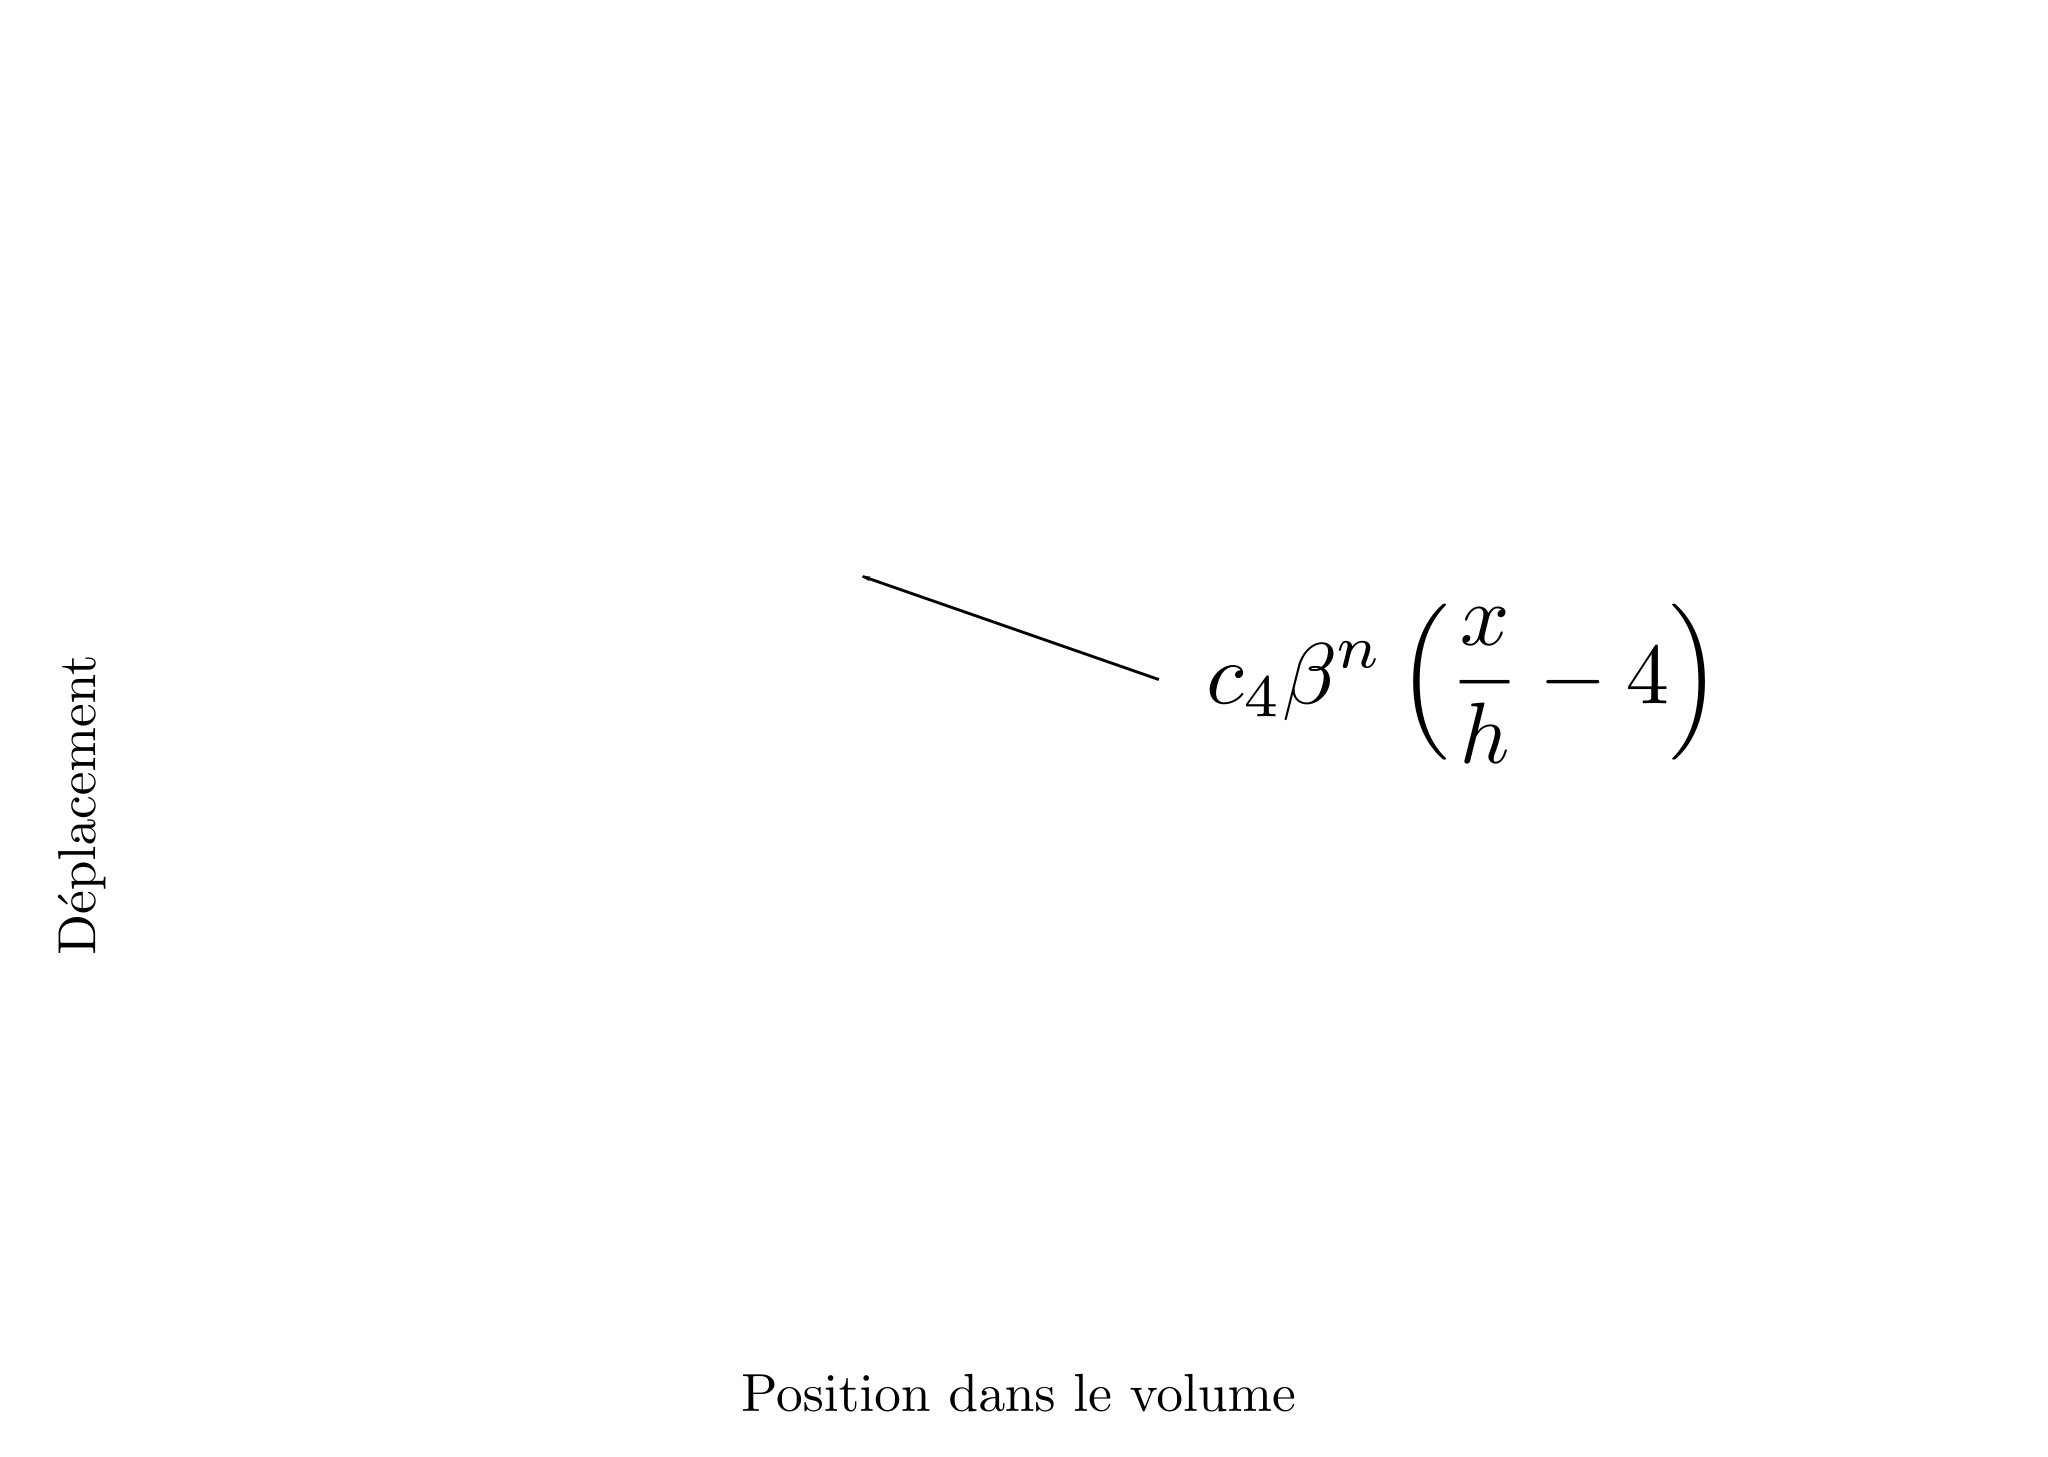
\includegraphics[width=17cm]{images/Bspline}
\caption[Exemple d'interpolation par B-spline]{Exemple d'interpolation par B-spline en 1 dimension : La courbe en trait pointillé épais est représentée par la la somme des contributions des courbes B-spline représentées en traits pointillés fins. Les points de la grille utilisée pour le placement des courbes sont représentés par les ronds rouge.}
\label{fig:Bspline}
\end{figure}


\begin{equation}
  g_t(x)=x + \sum\limits_{j\in \mathbb{Z}^N} c_j \beta^n \left( \frac{x}{h}-j \right)
\end{equation}

Où $\beta^n(x)$ est la valeur de la fonction B-spline de degré $n$ au point $x$, et $j$ représente les indices des positions de la grille. Le paramètre $h$ correspond à l'espacement entre les points de la grille. A chaque fonction B-spline de la grille correspond un coefficient de pondération associé nommé $c_j$ qui représente l'apport de la B-spline correspondante au signal final.

Les coefficients $c_j$ sont obtenus à l'aide d'une optimisation multi-échelle sur 3 niveaux : L'estimation est réalisée sur des images de résolution différente, en se basant sur l'estimation à la résolution $r-1$ pour réaliser celle de l'estimation à la résolution $r$. l'optimisation est réalisée par gradient conjugué selon la méthode de Polak-Ribière~\cite{polak1969note}. Nous avons utilisé l'erreur quadratique moyenne pour comme métrique de recalage. Elle a l'avantage d'être simple, rapide, et de ne pas montrer de discontinuités~\cite{ledesma2005spatio}. Nous avons choisi d'utiliser des splines d'ordre 1.


\subsection{Paramètres de l'estimation de mouvement}

%Les images utilisées pour l'estimation du mouvement respiratoire ne sont pas reconstruites avec les mêmes paramètres que les images finales. En effet, la quantité de données disponible pour la reconstruction est 8 fois plus faible que celle utilisée pour réaliser les reconstructions d'images. De plus, nous cherchons à optimiser la qualité de l'estimation de mouvement. 

L'estimation du champ de mouvement est réalisée à partir des 8 images TEP correspondant aux 8 positions temporelles du cycle respiratoire. Ces données contiennent donc 8 fois moins d'évènements que les images statiques. Ainsi, les paramètres de reconstruction déterminés en~\ref{lab:paramRecon} ne sont pas optimaux pour ces images, d'autant que nous cherchons, à ce stade, à optimiser la qualité de l'estimation de mouvement. C'est pour ces raisons que nous avons réalisé une autre étude pour estimer les paramètres de reconstruction pour cette problématique spécifique. 


\subsubsection{\'Evaluation de l'estimation de mouvement}

Pour évaluer la performance de chaque jeu de paramètre, nous avons utilisé la vérité terrain fournie par la carte de labels pour créer une image d'évaluation correspondant à l'image de référence, ainsi qu'une autre correspondant à l'image ``respirante``. Les images d'évaluation sont créées à partir des fantômes de référence en assignant aux organes étudiés (foie et poumon) une valeur de 1, et une valeur plus importante pour les lésions. Le reste a une valeur de 0. Une illustration est présentée dans la figure~\ref{lab:illustrationRecalage}.a). 

\begin{figure}
\centering
\begin{tabular}{c c}
	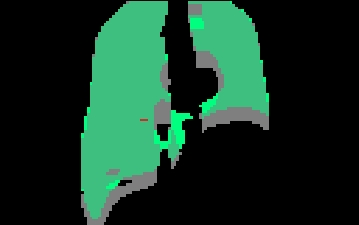
\includegraphics[width=5cm]{images/sansCorrection} & 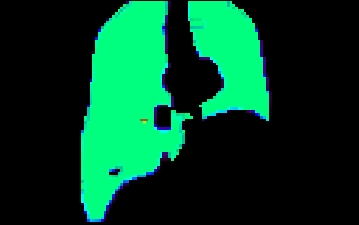
\includegraphics[width=5cm]{images/avecCorrection} \\
	a) Cartes non recalées				& b) Cartes recalées
\end{tabular}
\caption[Illustration du recalage obtenu]{Illustration de la pertinence du recalage obtenu à partir de l'estimation de mouvement réalisée sur les images. En vert l'image de référence et en gris l'image du temps correspondant à la différence la plus importante. }
\label{lab:illustrationRecalage}
\end{figure}

L'image d'évaluation correspondant à l'image ''respirante`` est alors recalée sur l'image de référence à l'aide du champ de mouvement élastique calculé précédemment. Nous évaluons ensuite la qualité du recalage en calculant l'écart quadratique moyen entre les deux images d'évaluation~\ref{lab:illustrationRecalage}.b).

\subsubsection{Optimisation des Paramètres de l'estimateur de mouvement}

Nous avons évalué l'influence de l'échantillonnage spatial des B-spline sur la qualité de l'estimation de mouvement. En effet, si l'espacement entre les nœuds de contrôle est trop important, les mouvements locaux vont interférer entre eux et le résultat ne sera pas valide. De la même manière, en cas d'espacement trop faible, la nature extrêmement bruitée des images va engendrer des micro-mouvements parasites locaux. Pour réduire le bruit, nous appliquons un filtrage gaussien de largeur à mi-hauteur égale à 6 mm à chaque itération.

Nous avons évalué le recalage des reconstructions pour les paramètres suivants :
\begin{description}
 \item[Nombre d'itérations :] Le nombre de sous-ensembles est toujours de 5, mais nous faisons varier le nombre d'itérations de 1 à 7, ce qui représente un nombre d'itérations totales de 5 à 40.
 \item[Précision de la grille :] nous avons évalué les performances de la détection pour 3 taille différentes, allant d'une grille très peu précise de 2 noeuds en x, y et z, à une grille plus précise avec 5 noeuds en x et y, et 10 noeuds en z. Une grille intermédiaire a été évaluée avec 3 noeuds en x et y, ainsi que 5 noeuds en z.
\end{description}

Les résultats sont présentés dans la figure~\ref{fig:perfsFctIterTaille}. Les meilleures performances sont obtenues pour la configuration $3 \times 3 \times 5$ avec 3 itérations et 5 sous-ensembles.

\begin{figure}
\centering
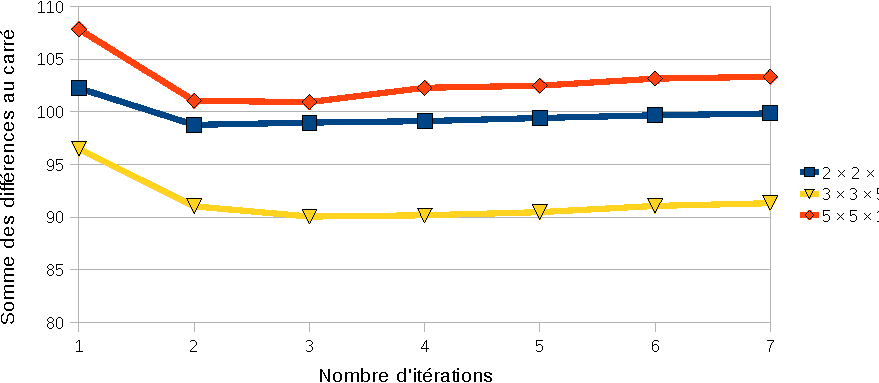
\includegraphics[width=12cm]{images/perfsRecalageFctIter-grid_crop}
\caption[Performances de l'estimation de mouvement en fonction de la taille de la grille de recherche]{Performances de l'estimation de mouvement en fonction du nombre d'itérations de la reconstruction selon la taille de la grille utilisée pour l'estimation de mouvement}
\label{fig:perfsFctIterTaille}
\end{figure}

\subsubsection{Optimisation des paramètres de la reconstruction}

Nous avons ensuite souhaité vérifier que la régularisation avait un impact positif sur la qualité du recalage. Nous avons utilisé les paramètres présentés précédemment pour la valider :

\begin{description}
 \item[Nombre d'itérations :] Le nombre de sous-ensembles est de 5, mais nous faisons varier le nombre d'itérations de 1 à 7, ce qui représente un nombre d'itérations totales de 5 à 40.
 \item[Présence ou absence de régularisation pendant la reconstruction :] Une régularisation par filtrage gaussien de largeur à mi-hauteur de 6 mm est appliquée ou non à chaque itération.
\end{description}

Les résultats sont présentés dans la figure~\ref{lab:perfsFctIterReg}. Ils montrent clairement que la régularisation entraîne une amélioration des performances, et que la meilleure estimation de mouvement est réalisée pour une reconstruction de 3 itérations avec 5 sous-ensembles. Nous avons par conséquent utilisé ces paramètres avec une grille de 3 noeuds en x et en y, soit un espacement de 17cm, et de 5 noeuds en z, soit un espacement de 7.7 cm.

\begin{figure}
\centering
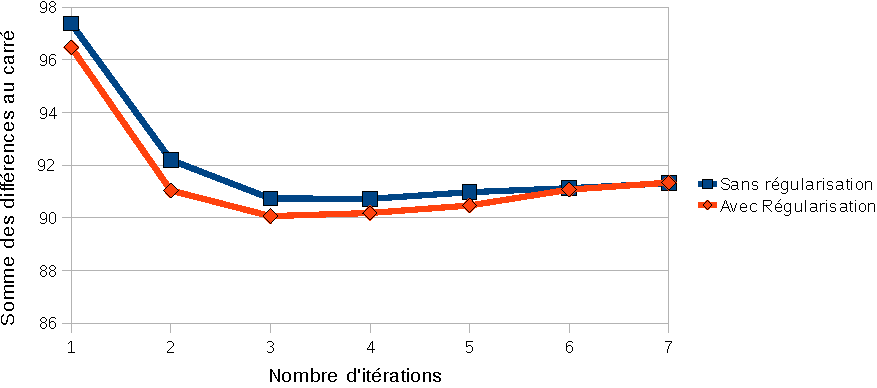
\includegraphics[width=10cm]{images/perfsRecalageFctIter_crop}
\caption[Performances de l'estimation de mouvement en fonction de la régularisation]{Performances de l'estimation de mouvement en fonction du nombre d'itérations complètes de la reconstruction selon la présence ou l'absence de régularisation pendant la reconstruction. Plus la valeur en ordonnées (mesure de différence) est faible, meilleure est la performance}
\label{lab:perfsFctIterReg}
\end{figure}


\section{Méthodes de correction du mouvement respiratoire}

Nous avons choisi de corriger les images TEP en utilisant la méthode de correction post reconstruction décrite en \ref{lab:corrPostRecon} ainsi que la correction par modification de la matrice système décrite en \ref{lab:corrMatSyst}. La première est déjà implémentée sur les imageur GE (technologie motionFree), tandis que la seconde est activement étudiée en recherche. Des images générées sur deux patients sont présentées dans la figure~\ref{fig:exempleImageReconTous}.

\begin{figure}
 \centering
 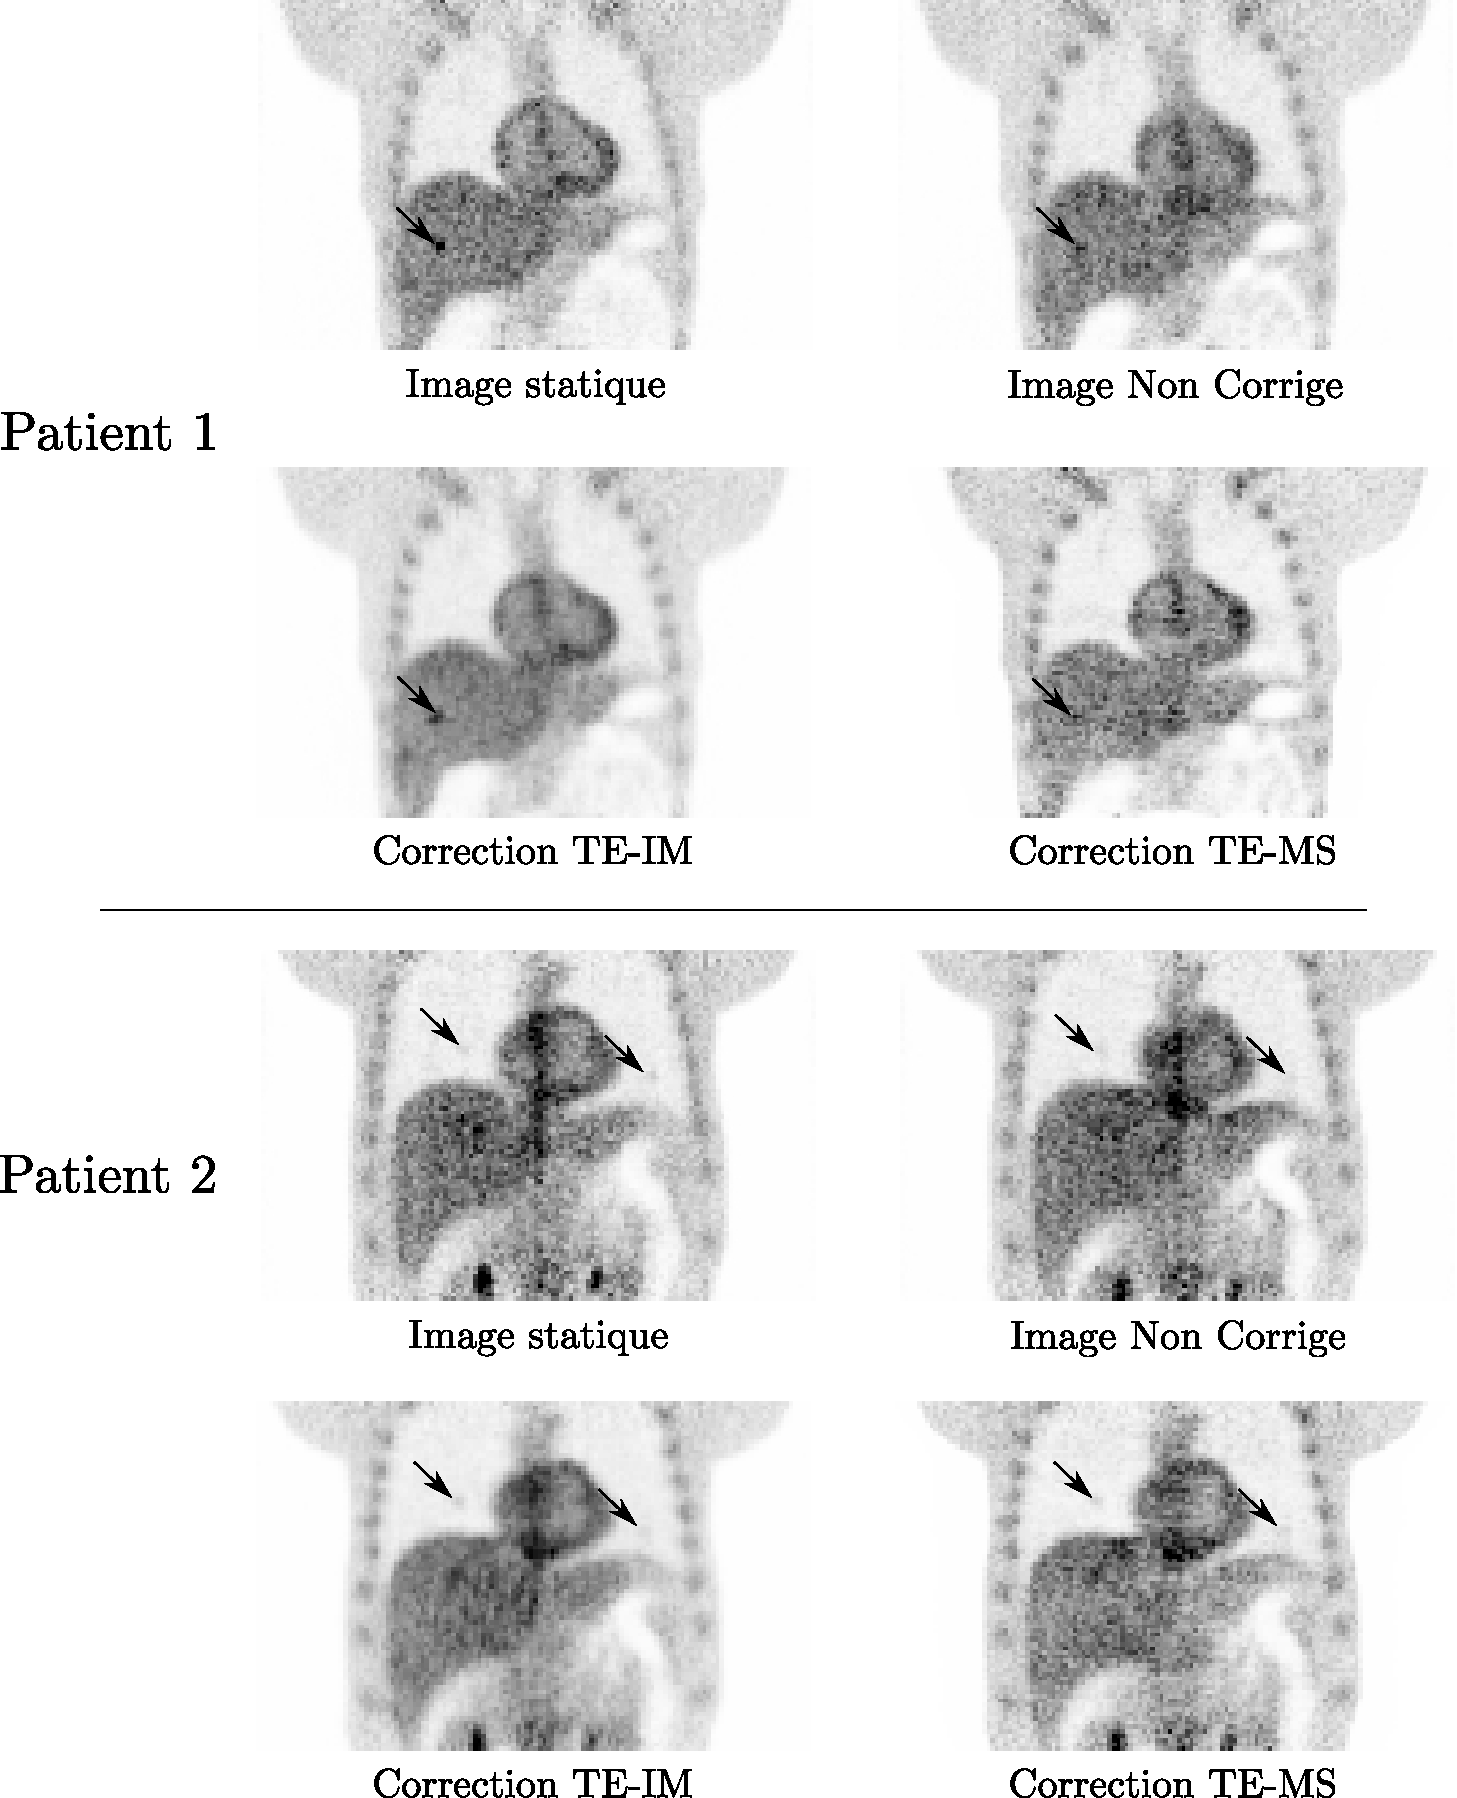
\includegraphics[width=15cm]{images/exempleImageReconToutes}
 \caption[Exemples d'mages reconstruites corrigées et non corrigées du mouvement]{Images reconstruites avec et sans correction du mouvement respiratoire (8 itérations et 5 subsets). Les flèches représentent une lésion du foie de diamètre 8 mm avec un contraste de 3.5 dans le patient 1, ainsi que deux lésions du poumon de 8 mm et de contraste 6.5 pour le patient 2.}
 \label{fig:exempleImageReconTous}
\end{figure}


\subsection{Images Statiques}

Les images statiques sont reconstruites à partir des données de simulation statiques, réalisées à partir d'une acquisition complète du modèle au premier instant du cycle respiratoire (fin d'expiration).

Chaque image est donc en phase avec la carte d'atténuation qui est elle aussi tirée du modèle en fin d'expiration. Les images ont été reconstruites à l'aide de l'algorithme OPL-EM avec 8 itérations comprenant 5 sous-ensemble chacune.

\subsection{Images Non corrigées}

Les images non corrigées sont produites de la même manière que les images statiques, mais à partir des fichiers séquence dynamiques. Ces fichiers correspondent à une acquisition en respiration libre de 224 secondes. 

La carte d'atténuation utilisée est celle correspondant au premier instant du cycle respiratoire.

\subsection{Images TE-MS}

Ces images sont reconstruites en utilisant la méthode décrite en~\ref{lab:CorrpendantRecon}, qui prend en compte l'estimation de mouvement réalisée précédemment ainsi que les fichiers séquence générés par la simulation dynamique pour reconstruire directement les images corrigées. 

La carte d'atténuation de l'instant de référence est déformée à l'aide des champs de mouvement pour générer 8 cartes d'atténuation. Les données de chaque instant du cycle respiratoire seront corrigées avec la carte d'atténuation correspondante.

\subsection{Images TE-IM}

La méthode TE-IM est présentée en~\ref{lab:corrPostRecon}. Les 8 images correspondant aux 8 instants du cycle moyen sont reconstruites séparément à l'aide de la carte d'atténuation recalée correspondante. Chacune de ces image est recontruite avec les mêmes paramètres que pour les autre types d'images, soit 8 itérations et 5 subsets. Ces 8 images sont ensuite déformées sur l'image correspondant au premier instant du cycle, à l'aide de la carte de mouvement estimée précédemment. Ces 8 cartes recalées sont ensuite sommées pour obtenir les images corrigées.

Bien que chaque image prise indépendamment soit très bruitée à cause du faible nombre d'évènements, la déformation suivie par la sommation des différentes images apporte une régularisation importante, comme on peut le voir dans la figure~\ref{fig:exempleImageReconTous}. 

\section{Système CAD} % 11.1

Le système CAD que nous utilisons a été développé à l'origine pendant les travaux de thèse de Sandrine Tomeï ainsi que mes travaux de master~\cite{tomei2008automatic,lartizien2010impact}. Nous l'avons amélioré et adapté aux besoins de cette étude, notamment en développant les mesures de performances.


Le CAD utilise des informations fréquentielles obtenues par décomposition des images en ondelettes biorthogonale 4/4 non décimée (figure \ref{fig:ondelettes}) . Ces données sont utilisées par le système de classification basé sur un SVM travaillant voxel par voxel. Une étape de réduction des faux positifs est ajoutée par la suite.

Le nombre de tumeurs utilisées pour générer la base d'apprentissage est de 107 pour la base d'apprentissage poumon et 173 pour la base d'apprentissage foie. Ce nombre est relativement faible~\cite{hua2005optimal} par rapport à la taille du vecteur de caractéristiques utilisé pour le CAD (entre 24 et 32), ce qui nécessite de prendre en compte un maximum de données pour l'apprentissage et le test pour éviter le sous-apprentissage. Nous avons donc utilisé une méthode d'évaluation des performances par resubstitution. Cela signifie que les apprentissages et les tests sont réalisés sur la même base de données constituée de 15 patients présentés dans le chapitre 10. %\ref{lab:bdd}.

\subsection{Vecteur de Caractéristiques}

Nous avons choisi d’utiliser une décomposition en ondelettes 3D non décimées par banc de filtres. Dans le cas tridimensionnel, la décomposition par banc de filtres est résumée par la figure \ref{fig:ondelettes}. L’image de départ est traitée successivement dans les trois directions de l’espace par un filtre fréquentiel passe-haut correspondant à la fonction d’ondelettes (noté $H$) et passe-bas correspondant à la fonction d’échelle (noté $L$). 

\begin{figure}
 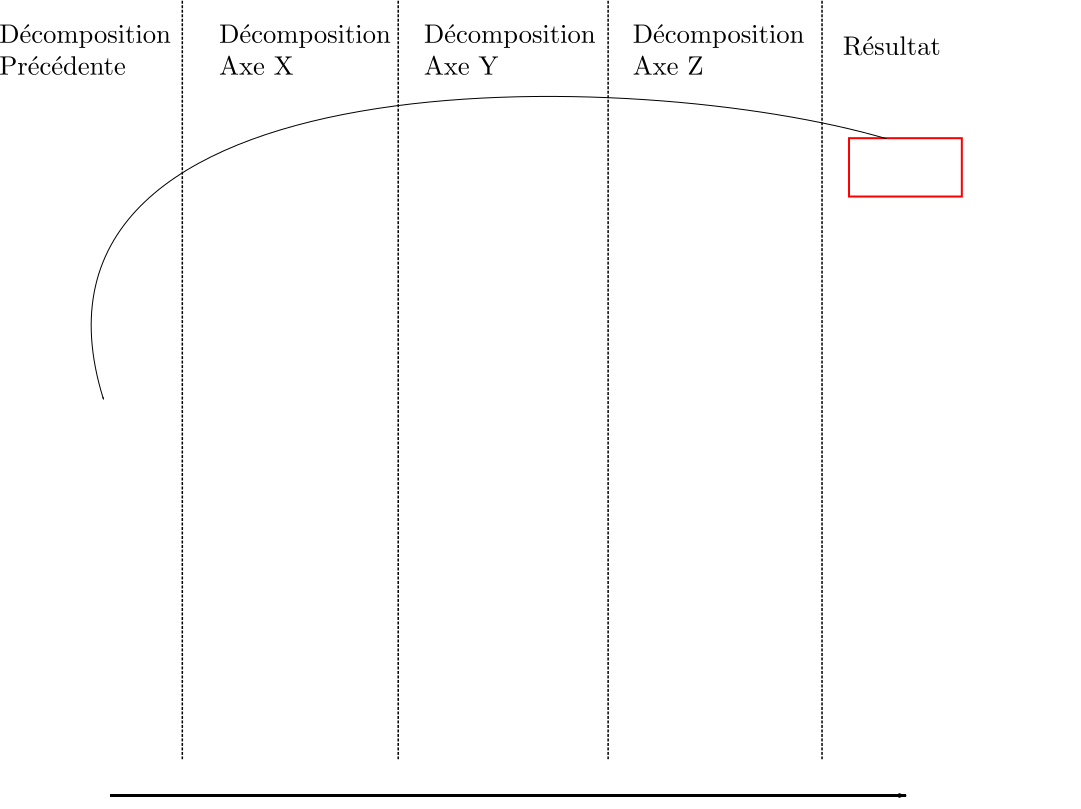
\includegraphics[width=15cm]{images/decompHotell}
 \caption[Décomposition en ondelettes par banc de filtres]{Décomposition en ondelettes par banc de filtres : Chaque image est filtrée selon les 3 dimensions pour obtenir les coefficients d'ondelettes et d'échelle de chaque voxel de l'image. L correspond à un filtrage passe-bas tandis que H correspond à un filtrage passe-haut. Les coefficients d'échelle sont contenus dans l'image $LLL_{j+1}$ tandis que les coefficients d'ondelettes sont présents dans les sept images de détail $LLH_{j+1}$, $LHL_{j+1}$ \dots $HHH_{j+1}$ }
 \label{fig:ondelettes}
\end{figure}

\begin{figure}
 \centering
 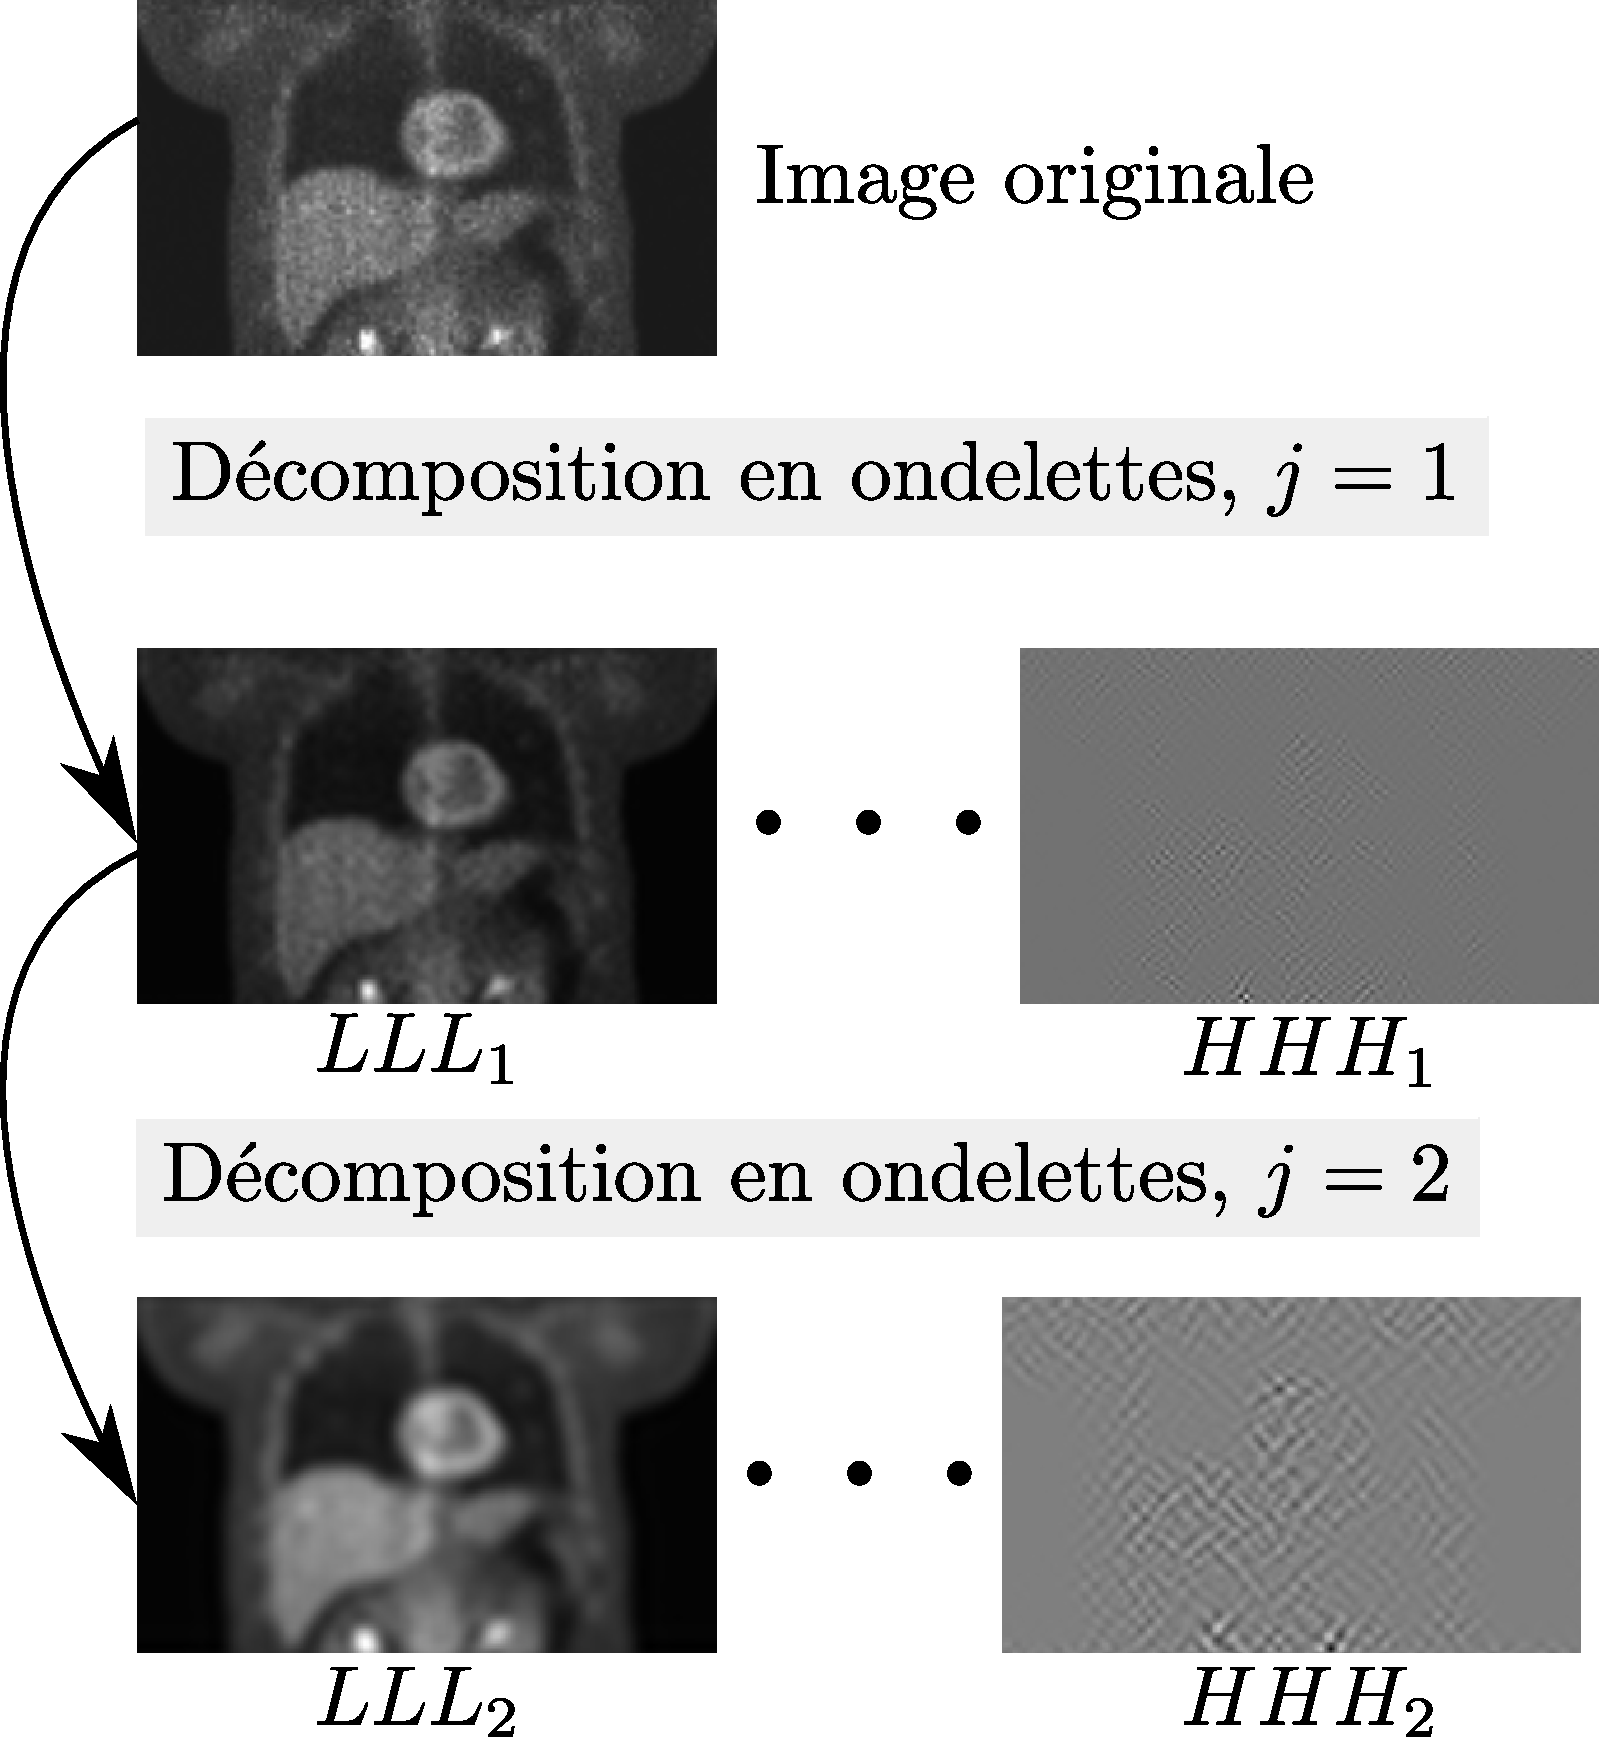
\includegraphics[width=15cm]{images/exemplesDecomp}
 \caption[Exemples de décomposition d'images en ondelettes]{Exemples d'images TEP décomposées en ondelettes. Sont représentées l'image originale, puis l'image des coefficients d'échelle notée $LLL_j$ et une image des coefficients d'ondelettes notée $HHH_j$ pour deux niveaux de décomposition. L'ondelette utilisée pour la décomposition est la biorthogonale 4/4}
 \label{fig:bior44Ex}
\end{figure}


Ainsi sept images de détails (HHH, LLH, \dots) et une image d’approximation (LLL) sont produites pour chaque niveau $j$ de décomposition. Les huit images du niveau suivant $j+1$ sont générées de la même manière, mais en considérant l’image d’approximation $LLL_j$ du niveau précédent comme image de départ. Les caractéristiques des images, rassemblées dans un vecteur descripteur de taille $8 \times j$, correspondent ici à l’ensemble de ces coefficients pour chaque voxel  de l’image. Des exemples d'images obtenues par les filtrages sont présentés dans la figfure \ref{fig:bior44Ex}.

Nous utilisons l'ondelette biorthogonale 4/4 dont la fonction est présentée sur la figure \ref{fig:bior44}.


\begin{figure}
 \begin{tabular}{ c c }
 
 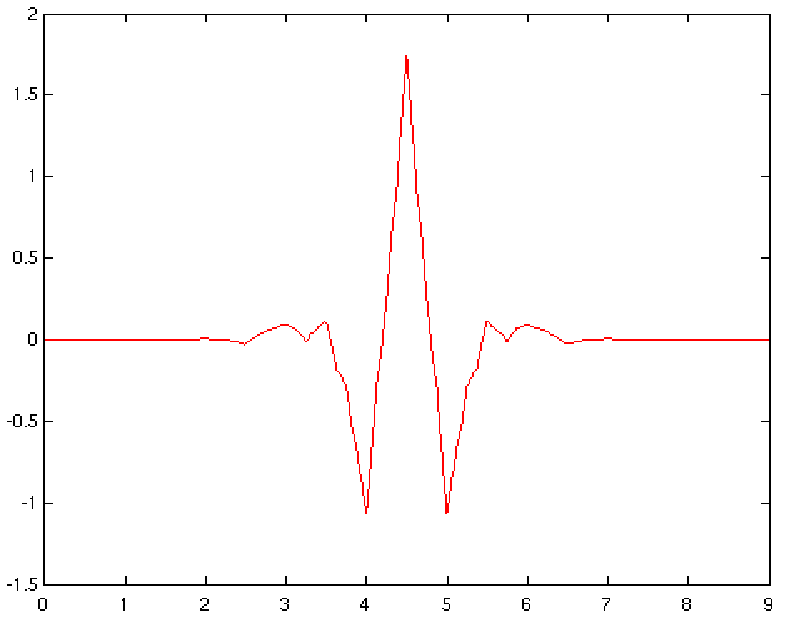
\includegraphics[width=8cm]{images/bior44Ondelette} & 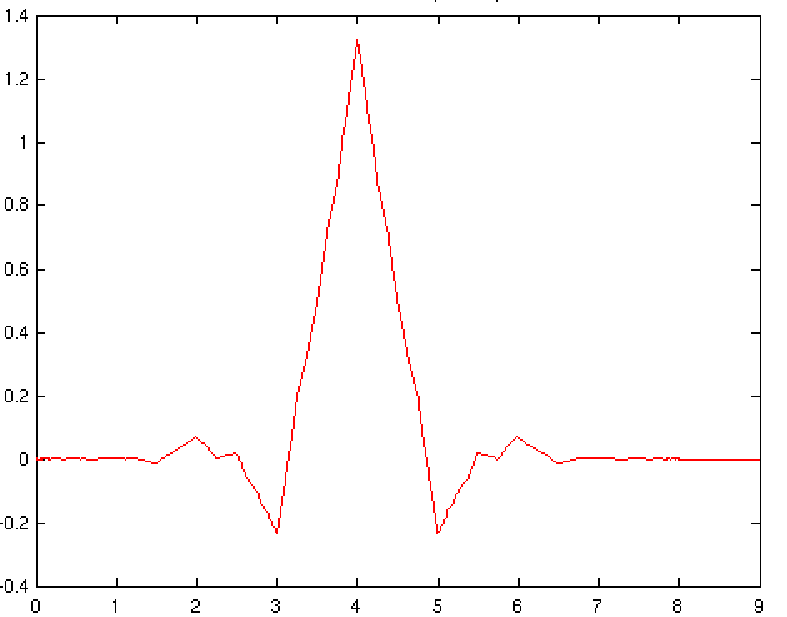
\includegraphics[width=8cm]{images/bior44Echelle} \\
 Fonction d'ondelette & Fonction d'échelle\\
 \end{tabular}

 \caption{Fonction d'ondelette et d'échelle biorthogonale 4/4}
 \label{fig:bior44}
\end{figure}

\subsection{Génération de la base d'apprentissage}
Les données générées par la décomposition en ondelettes de chaque image se présentent sous la forme de volumes 4D, indiquant pour chaque voxel de l'image 3D l'ensemble des $8 \times j$ coefficients associés.

La base d'apprentissage sert à entraîner le classifieur dans un processus de classification supervisée, en lui fournissant un ensemble d'exemples avec leur classes associées (voir figure \ref{fig:fonctClassif}) page \pageref{fig:fonctClassif}).

La génération de cette base demande l'extraction de points de la classe ``pathologique'', et de la classe ``sain''. Pour chaque tumeur de la vérité terrain, nous extrayons de l'image correspndante le vecteur de caractéristiques du voxel placée au centre de la tumeur. Ce vecteur de caractéristique correspond aux coefficients de la décomposition en ondelette du voxel de l'image ($8 \times j$).

Les points de la classe ``sain'' sont extraits de manière aléatoire dans les volumes de toutes les images (hors tumeurs). Pour des raisons de simplicité d'implémentation, un nombre fixe de points est extrait de chaque image.

\subsection{Apprentissage de la Machine à Vecteur de Support (SVM)}

La base de données d'apprentissage est utilisée  par le classifieur SVM (Machine à Vecteur de Support) pour l'apprentissage.

Le principe des SVM est de trouver l’hyperplan optimal de séparation dans l'espace des caractéristiques, qui va maximiser la marge de séparation entre les deux classes ``pathologique''  et ``sain'' (le SVM est défini plus en détail en \ref{lab:SVM}). Cette marge correspond à la distance entre les plus proches vecteurs de caractéristiques appartenant à chacune des classes et l'hyperplan. La définition de cette marge et donc de l’hyperplan, se fait uniquement à partir de vecteurs de support, qui correspondent à l'enveloppe du groupement de point de chacune des deux classes.

Le SVM va calculer un modèle décrivant l'hyperplan permettant de séparer les données.

\subsection{Génération des sites présumés}
\label{lab:aggregatsCAD}
Une fois le classifieur entraîné, il est capable de classer rapidement les nouveaux vecteurs de caractéristiques. Ainsi, on lui soumet les données correspondants aux voxels des images pour qu'il les classe. On obtient donc en sortie un ensemble de cartes de score (une par image 3D), dans lesquelles chaque voxel correspond au score indiqué par le SVM. Ce score est une mesure de distance polarisé par rapport à l'hyperplan de séparation dans l'espace des points d'apprentissage, et donne en plus de la classe, une mesure assimilable à la confiance du SVM vis-à-vis de sa classification.

Cette carte de score est ensuite seuillée pour fournir une carte binaire, indiquant pour chaque voxel la classe sélectionnée par le SVM pour ce niveau de seuil. Le mécanisme de sélection du seuil est défini en \ref{lab:selectionSeuil}. Une exemple de carte de score est visible dans la figure \ref{fig:cheminementCAD}.a.
	
\`A cette étape, le résultat est sous forme d'une carte de voxels étiquetés comme ''sain`` ou ''pathologiques``. Nous avons choisi de travailler sur des agrégats de points plutôt que directement sur les voxels car les cartes binarisées sont relativement bruitées (voir \ref{fig:cheminementCAD}.b), et donc non directement exploitables. Les voxels ``pathologiques'' sont donc regroupés selon une 26-connexité (3x3x3). Un score est associé à chaque  agrégat, correspondant au score le plus important observé dans l'agrégat.

\subsection{Règles d'évaluation du résultat}
\label{lab:reglesSelect}
Pour évaluer le résultat, nous avons élaboré des règles permettant de classer les agrégats à l'aide de la vérité terrain. Ce sont ces algorithmes qui sont utilisés dans les évaluateurs de performances présentés ci-après.

Les agrégats sont classés en LL (Lésion localisée) et NL (Non Lésion) selon qu'ils peuvent être considérés comme des vrais positifs ou des faux positifs :

Soit $\mathbf{L}$ l'ensemble des points de la lésion, $\mathbf{A}$ les points correspondant à l'amas candidat.

Les agrégats seront considérés comme des vrai positifs si ils intersectent une tumeur selon les règles décrites ci-après, ou comme de faux positifs dans le cas contraire. Cependant, si leur taille est inférieure à la taille minimale définie par la première règle, l'amas n'est pas considéré.

Règles de classification :
\begin{enumerate}
 \item $card( \mathbf{L} \cap \mathbf{A} ) > \alpha \times card( \mathbf{L} )$ : où $\alpha$ définie la proportion minimale de la tumeur qui doit être présente dans l'amas. Elle permet d'éviter les amas qui intersecteraient la tumeur par accident.
 \item $card( \mathbf{L} \cap \mathbf{A} ) > \beta \times card( \mathbf{A} )$ : où $\beta$ limite l'étendue de l'amas en dehors de la tumeur.
\end{enumerate}

$\alpha$ et $\beta$ sont des constantes empiriques fixées respectivement à 0.05 et 0.20 dans nos travaux. Nous avons choisi ces valeurs en visualisant les cartes de score pour obtenir des résultats corrects sans pénaliser les performances.

\subsection{Résumé}

Ce pseudo-code décrit les différentes étapes du CAD, depuis l'importation des images jusqu'à à l'extraction des lésions potentielles. Il est illustré par la figure \ref{fig:cheminementCAD} :

\begin{figure}
 \centering
 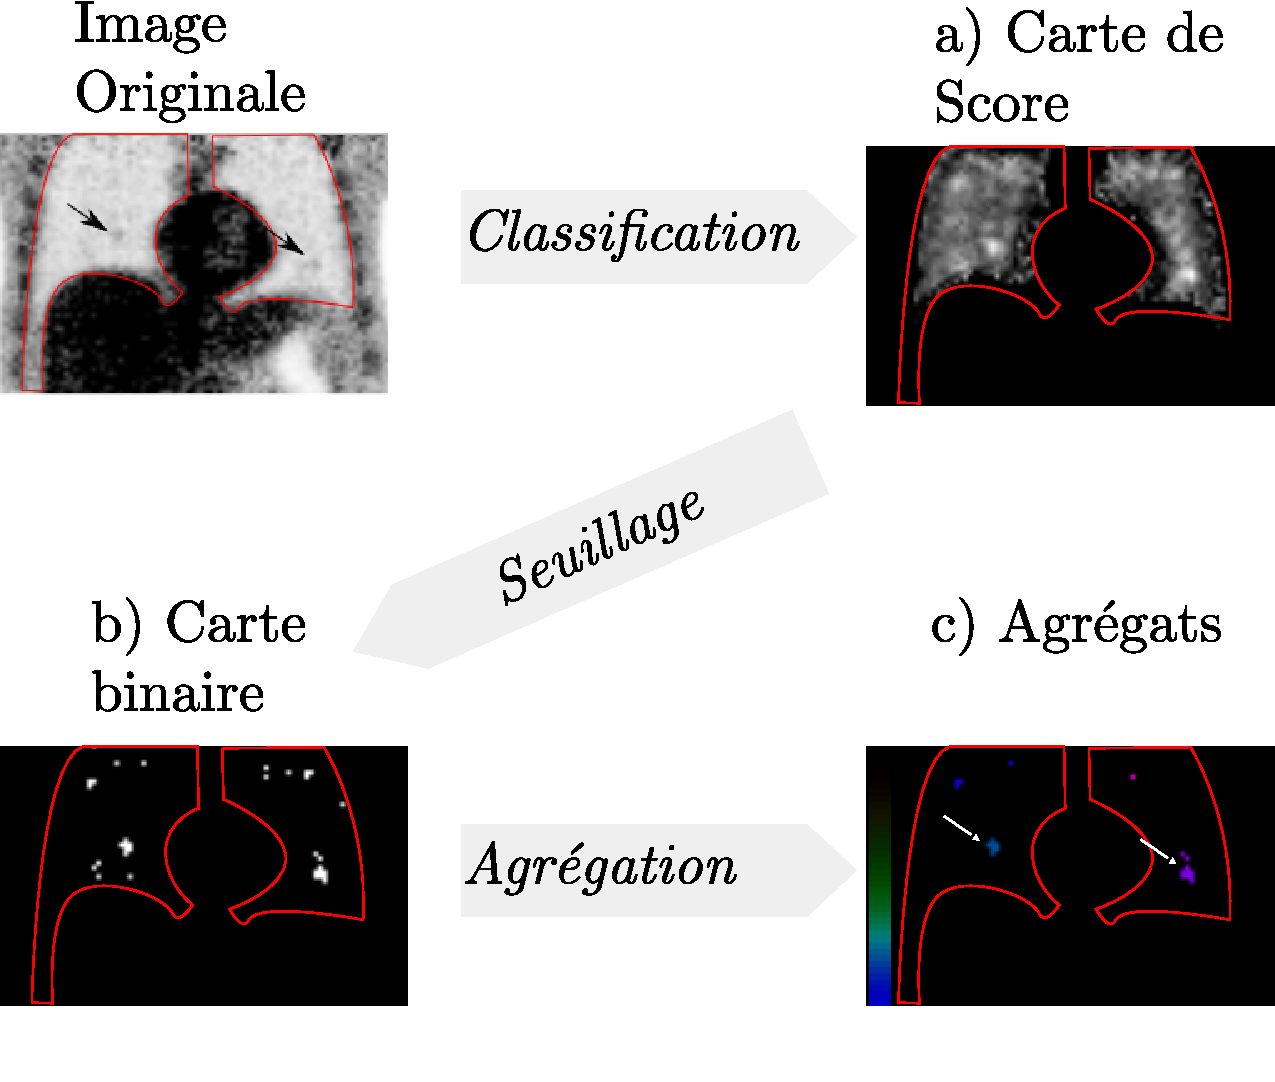
\includegraphics[width=15cm]{images/cheminementCAD}
 \caption[Schéma du système CAD]{Schéma du système CAD : l'image d'origine en haut à gauche est utilisée par le classifieur pour générer la carte de score. Cette carte est ensuite seuillée par l'étape b) pour générer une carte binaire correspondant aux sites qui dépassent un certain score $s$. L'étape c) correspond à la formation des agrégats qui seront le résultat du système CAD. Cette étape s'accompagne d'une suppression des sites de trop petite taille. Les flèches représentent des lésions dans l'image d'origine}
 \label{fig:cheminementCAD}
\end{figure}

\begin{enumerate}
 \item Décomposition des images en ondelettes : pour chaque voxel de l'image d'origine, on obtient entre 8 et 32 coefficients suivant le niveau de décomposition de l'image, qui correspondent au vecteur de caractéristiques utilisé par le classifieur.
 \item Extraction de la base d'apprentissage : les coefficients des centres de toutes les tumeurs sont extraits des volumes décomposés, et vont former la base d'apprentissage pathologique. Un certain nombre de voxels sont tirés aléatoirement dans les zones normales de chaque image et leurs coefficients sont ajoutés à la base saine.
 \item Apprentissage : le classifieur SVM est entraîné sur cette base d'apprentissage pour générer le modèle qui sera utilisé pour le test.
 \item Tests : le SVM entraîné est utilisé pour classer chaque voxel contenu dans les organes à évaluer (poumon et foie).
 \item Réduction des faux-positifs : les points sont agrégés en composantes connexes (26-connexité en 3 dimensions).
 \item Évaluation : lorsque nous avons accès à la vérité terrain, il est possible d'évaluer les performances du CAD en classant les agrégats en LL (Lésion Localisée) et LN (Lésion Non Localisée).
\end{enumerate}



\section{Optimisation des paramètres du système CAD} % 11.2
\label{lab:optim}

Les différentes étapes de l'évaluation des performances nécessitent de fixer un grand nombre de paramètres que nous allons détailler dans cette partie.

\subsection{Paramètres à optimiser} % 11.2.1
\label{lab:optimParametres}

\subsubsection{Paramètres de la base d'apprentissage}

Nous avons identifié plusieurs autres paramètres qui, sont suceptible d'influencer les performances de détection :

\begin{enumerate}
 \item \textbf{Normalisation :} Le but de la normalisation est d'homogénéiser les plages de valeurs des différentes caractéristiques pour faciliter le travail du classifieur, dont les paramètres $C$ et $\gamma$ (définis ci-après) dépendent de la distance entre les points et ne permettent pas de gérer des différences trop importantes d'étendues dans les caractéristiques.  Nous avons proposé de comparer deux méthodes de normalisation. La première consiste à modifier les données pour que la moyenne et l'écart-type aient une valeur respectivement de 0 et 1 ($(\mu, \sigma)=(0,1)$). Cette méthode est notée ``\emph{moyenne}'' dans la suite du texte. La seconde méthode consiste à adapter des données pour que l'ensemble des valeurs soit comprises entre -1 et +1. Cette méthode est notée ``\emph{écart}''. La première méthode (\emph{moyenne}) a l'avantage d'être relativement peu sensible aux valeurs extrêmes, contrairement à la seconde (\emph{écart}).


 \item \textbf{Nombre de points de la base d'apprentissage :} Le nombre de point de la base d'apprentissage détermine directement la qualité du modèle. Le nombre de caractéristiques de chaque exemple de la base est de $8 \times j$, avec $j$ le niveau de décomposition des images. Il n'existe pas de règle définitive pour choisir le nombre d'exemples nécessaires en fonction du nombre de caractéristiques, mais l'on considère cependant que le nombre d'échantillons de la base d'apprentissage doit être largement supérieur au nombre de caractéristiques pour éviter le sur-apprentissage. Cependant, les SVM sont relativement efficaces pour éviter ce problème. Dans notre étude, le nombre de cas pathologiques est de 173 pour le poumon et de 107 pour le foie. Il faudrait idéalement sélectionner autant de cas ``sains'' que de cas pathologiques pour chaque organe. Cependant le nombre total de cas risque d'être trop faible par rapport au nombre de caractéristiques. Nous avons par conséquent analysé l'influence du nombre de cas sur les performances de détection en considérant trois valeurs : 100 points normaux par images (pts/im.) (soit 1500 pts. négatifs), 200 pts/im. (soit 3000 pts. négatifs) et 1000 pts/im. (soit 15000 pts. négatifs).


 \item \textbf{positions des points extraits :} Les points normaux extraits des images pour alimenter la base vont avoir une influence directe sur la qualité des résultats. Idéalement ils devraient être représentatifs de l'ensemble des cas rencontrés dans la base de tests, néanmoins les bords de certains organes ont un profil proche de celui des tumeurs, et rendent l'estimation de la surface de séparation plus difficile. Nous avons donc voulu évaluer la performance du CAD sur une base dépourvue de ces données ambiguës. Pour cela nous avons réalisé une érosion de 2 voxels sur les masques des volumes sains à extraire, afin de ne pas prendre en compte les frontières des organes.
\end{enumerate}



\subsubsection{Paramètres du classifieur}
\label{lab:paramClassif}
Le classifieur (SVM) utilise les données d'apprentissage formatées selon les choix opérés précédemment (normalisation, volumes utilisés pour extraire les points de la base de points ''sain`` et nombre de ces points) pour générer un modèle de prédiction. Cependant, cet algorithme dispose de paramètres intrinsèques, qui sont beaucoup plus dépendant des données d'apprentissage (voir \ref{lab:SVM}).

\begin{description}
 \item[Niveau de la décomposition en ondelettes $j$ :] Ce paramètre détermine la taille du vecteur de caractéristiques. il correspond au nombre de niveaux de décomposition pris en compte par le SVM. Les niveaux de décomposition élevés ($j$ grand) correspondant à des informations de très basse fréquence, les informations qu'ils apportent ne sont pas forcément pertinentes pour la détection des lésions. Cependant, les caractéristiques fréquentielles des images générées par les différents jeux d'images étant différentes, il est nécessaire d'adapter ce paramètre à chaque type d'images.
 \item[Coefficient de pénalisation $C$ :] lors du calcul de l'hyperplan de séparation des données, chaque point mal classé va pénaliser la surface selon un facteur proportionnel à $C$, comme indiqué en~\ref{lab:SVM}.
 \item[Largeur de bande $\gamma$ :] cette valeur influe directement la largeur de bande du noyau utilisé par le classifieur (Fonction de Base Radiale gaussienne, ou RBF). Voir la description du SVM en~\ref{lab:SVM}
\end{description}

\subsection{Méthodes d'optimisation}
\label{lab:optimCGJ}

Pour chaque combinaison des paramètres de la base d'apprentissage définis en~\ref{lab:paramClassif}, nous avons déterminé le triplet optimal de paramètres ($C$, $\gamma$, $j$) à l'aide d'une recherche exhaustive par grille. Cela correspond à évaluer les performances sur le produit cartésien d'une discrétisation des valeurs de chaque paramètre. Cette étude a été réalisée sur le jeu d'images statiques afin de ne pas être influencé par les éventuels artefacts des autres types d'images.

Par exemple, si nous disposons de deux paramètres A et B, et que nous recherchons le meilleur jeu de paramètres, il faut tout d'abord sélectionner pour chaque paramètre la taille de la zone de recherche. Supposons par exemple que les valeurs de A soient des valeurs entières comprises entre -1 et 2, et que B puisse prendre les valeurs 100, 10000 et 50000. Les critères de performance seront évalués pour toutes les combinaisons des valeurs de A et B, tels que (-1, 100), (-1, 10000), (-1, 50000), (0, 100), \dots, (2, 50000). Le jeu de paramètres ayant obtenu les meilleures performances sera donc sélectionné. 

Les critères de performance que nous avons sélectionnés sont la sensibilité et la spécificité obtenue pour une validation croisée à 5 éléments réalisée sur la base d'apprentissage comme présenté sur la figure \ref{fig:crossValid}. La validation croisée permet de réduire le biais sur les performances~\cite{varma2006bias}.

\begin{figure}[h!]
 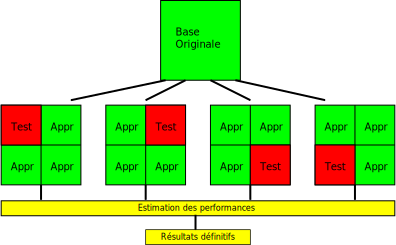
\includegraphics[width=15cm]{images/crossValid}
 \caption[Réalisation d'une validation croisée à $n$ éléments]{Réalisation d'une validation croisée à $n$ éléments (ici 4) : La base d'exemples d'origine est décomposée en $n$ parts égales. La mesure de performance se fait $n$ fois, avec à chaque fois un apprentissage sur $n-1$ éléments et un test sur l'élément restant. La mesure de performance est réalisée sur les résultats des $n$ tests.}
 \label{fig:crossValid}
\end{figure}


Pour choisir les meilleurs paramètres du classifieur, j'ai effectué une recherche exhaustive par grille avec les paramètres suivants :

\begin{description}
 \item [$C$ :] de 1 à 10000 en 15 pas logarithmiques
 \item [$\gamma$ :] de 0.0001 à 1 en 15 pas logarithmiques
 \item [$j$ :] de 1 à 4, soit de 8 à 32 caractéristiques
\end{description}

L'optimisation a été réalisée à l'aide du logiciel rapid-i~\cite{mierswa2006} pour chaque type d'image. Les indicateurs de performance calculés par validation croisée sont les suivants : sensibilité, spécificité et précision définis dans le chapitre 7 (section \ref{lab:pressensib}). Le triplet de paramètres retenu est celui qui maximise la sensibilité.

Nous avons représenté pour chaque jeu d'image le nuage de points correspondant à la répartition de chaque triplet ($C, \gamma, j)$ dans un espace à deux dimensions (``Sensibilité'', ``Spécificité''). De ce nuage de points nous pouvons voir le front de Pareto. Ce type de diagramme permet de rechercher un optimum selon plusieurs critères antagonistes. Dans notre cas, nous voulons à la fois une sensibilité et une spécificité importante, sachant qu'il n'existe pas de jeu de paramètres ''parfaits`` qui permettent d'avoir 100\% aux deux. Dans notre cas, le front de Pareto va permettre de vérifier que le choix par maximisation de la sensibilité ne se fait pas au détriment de la spécificité.


\subsection{Mesure de performances de détections}
\label{lab:selectionSeuil}
\label{lab:optimIMSTNOMS}
Les performances de détection obtenues par la méthode de validation croisée considère uniquement le voxel central de la tumeur
pour déterminer si la lésion est correctement détectée. Ces performances ne traduisent donc pas forcément le comportement d'un observateur humain, qui détecte plutôt des aggrégats. Nous avons donc proposé d'estimer les performances en considérant la notion d'aggrégats. Pour un seuil donné, le CAD génére un ensemble d'agrégats associés à un score, comme présenté en \ref{lab:aggregatsCAD}. Il est ensuite possible d'évaluer la performance de ce CAD à l'aide de courbes F-ROC décrites en \ref{lab:FROC} construites à l'aide de la vérité terrain.

Le seuil sélectionné $s$ pour générer les agrégats est celui qui maximise la Fraction de Localisation de Lésion (FLL : nombre de lésions localisées divisé par le nombre total de lésions), c'est à dire celui qui va permettre de détecter un maximum de lésions. 

Cette sélection est réalisée selon l'algorithme suivant :

Le processus d'estimation de la sensibilité pour un seuil $s$ se fait de la manière suivante. Les cartes de scores sont binarisées en fonction de $s$. Les agrégats sont estimés sur ces cartes binaires, en prenant en compte les informations provenant des cartes de score correspondantes pour attribuer un score à chaque agrégat. Ils sont ensuite classés en ''Lésion localisée`` (LL) ou ''Non Lésions`` (NL) à l'aide de la vérité terrain, selon les règles présentées en \ref{lab:reglesSelect}. Une valeur de sensibilité est calculée à partir de ces informations pour le seuil $s$.

Le seuil optimal retenu est celui qui maximise la sensibilité. Nous recherchons ce maximum pour 40 valeurs réparties de manière uniforme entre -2 et +2. Nous utilisons une recherche exhaustive car le résultat possède de nombreux minima locaux et le temps de calcul est faible (moins d'une heure pour les 40 valeurs).

Ce critère de sélection va naturellement engendrer un grand nombre de faux positifs, mais il faut garder à l'esprit qu'il sera utilisé pour réaliser des courbes F-ROC, qui indiquent une spécificité pour chaque nombre de faux positif en jouant sur un second seuil, toujours supérieur à celui retenu pour extraire les agrégats.

Le second critère utilisé pour comparer les bases d'apprentissage est la figure de mérite extraite de l'analyse JAFROC décrite en \ref{lab:AFROC}. Elle va comparer pour chaque image le score du faux positif le plus haut avec les score des vrais positifs de l'image. Pour cette étude, nous avons utilisé la version 4.0 du logiciel JAFROC.

\section{Comparaison des performances de détection des différentes méthodes de correction du mouvement respiratoire}

L'optimisation des paramètres décrits dans la section~\ref{lab:optimParametres} nous a permis de fixer les paramètres de la base d'apprentissage (normalisation, nombre de cas sains, localisation des cas sains).

Afin de comparer les performances des quatre séries (statique, non corrigéee, TE-IM et TE-MS) nous avons dans un premier temps réalisé une nouvelle optimisation des paramètres ($C$, $\gamma$, $j$) pour chaque type d'images en suivant la méthode décrite en~\ref{lab:optimCGJ}. Puis nous avons comparé les courbes F-ROC et réalisé une étude JAFROC comme décrit dans la section~\ref{lab:optimIMSTNOMS}



%%% CHAPITRE 12


\chapter{Analyse des résultats}

Dans ce chapitre nous détaillons les performances de détection obtenus par les quatre séries d'images que nous avons comparées : TE-IM, TE-MS, Statiques et Non Corrigées. Nous commençons par présenter les courbes obtenues lors de l'étape d'optimisation et d'adaptation du CAD aux données, puis nous parlons des performances de détection obtenues par ce CAD sur les lésions hépatiques et pulmonaires.

Dans tous les cas, l'estimation des performances se fait de la manière suivante :

\begin{itemize}
 \item Optimisation des paramètres du classifieur au jeu de données.
 \item Comparaison des courbes Free-ROC.
 \item Comparaison des Figures de Mérite JAFROC.
 \item Conclusion
\end{itemize}


\section{Optimisation des paramètres}

Nous avons réalisé des mesures de performances pour les différentes valeurs des paramètres suivants :

\begin{itemize}
 \item Nombre de points de la base d'apprentissage (100, \textbf{200}, 1000)
 \item Normalisation des données (\textbf{moyenne}, écart)
 \item Position des points de la base d'apprentissage (\textbf{organe complet}, organe avec érosion)
\end{itemize}

La recherche des paramètres optimaux a été réalisée sur le foie, pour la série d'images statiques, afin de ne pas être influencé par les artefacts des méthodes de correction du mouvement respiratoire. Pour sélectionner le jeu de paramètre optimal, nous avons créée une base \textbf{Témoin} comprenant les valeurs en gras des paramètres présentés ci-dessus. Toutes les autres bases reprennent les valeurs de la base Témoin en modifiant un seul paramètre. Nous utiliseront par la suite les termes définis ci-dessous pour qualifier les 5 jeux de paramètres :

\begin{description}
 \item[Base Témoin : ] contient des données normalisées par la méthode ''moyenne`` avec 200 points sains extraits de chaque ensemble du volume des organes.
 \item[Base Érodée : ] contient des données normalisées par la méthode ''moyenne`` avec 200 points sains extraits du volume de chaque organe érodé (érosion morphologique de 2 voxels).
 \item[Base Appauvrie : ] contient des données normalisées par la méthode ''moyenne'' avec 100 points sains extraits de l'ensemble du volume de chaque organe.
 \item[Base Enrichie : ] contient des données normalisées par la méthode ''moyenne`` avec 1000 points sains extraits de l'ensemble du volume de chaque organe.
 \item[Base Normalisée \'Ecart : ] contient des données normalisées par la méthode ''écart`` avec 200 points sains extraits de l'ensemble du volume de chaque organe.
\end{description}

Pour vérifier que les résultats de la sélection des paramètres du classifieur sont stables, une seconde base témoin (\textbf{Témoin 2}) a été générée avec les données de seulement 14 images sur les 15 que nous avons simulées. Les points ''sains`` ne sont pas non plus extraits aux mêmes endroits que pour la base \textbf{Témoin}. Nous allons donc vérifier que les paramètres optimaux du CAD pour un jeu de données ne sont pas dépendants de la base.

\subsection{Sélection des meilleurs paramètres du classifieur}
\begin{figure}[h!]
\begin{center}
 
\includegraphics[width=14cm]{images/pareto_param_200}

{\small a) Base Témoin}
\vspace{0.5cm}

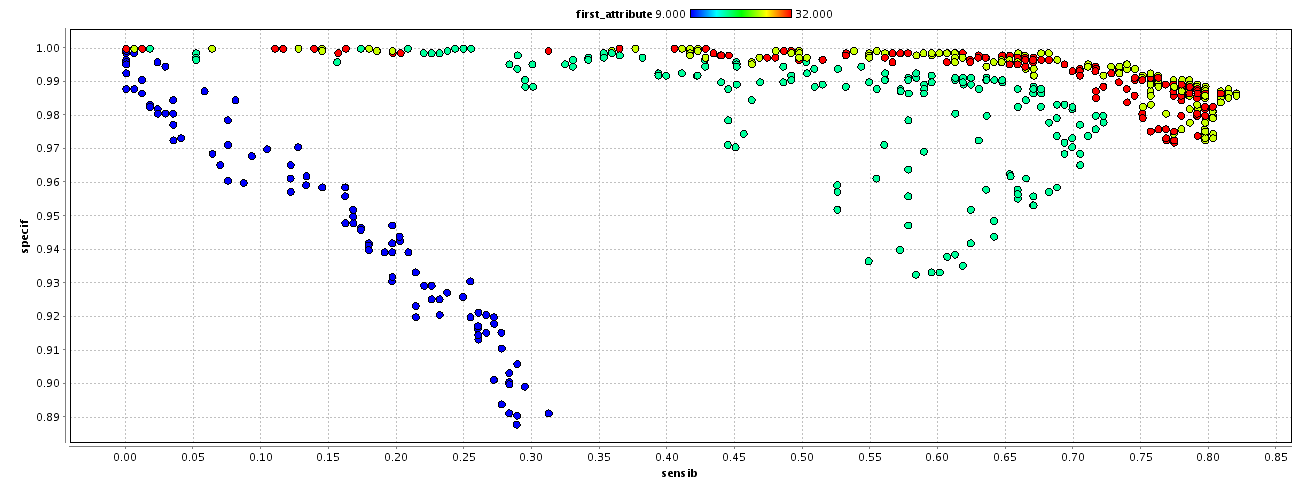
\includegraphics[width=14cm]{images/pareto_param_100}

{\small b) Base appauvrie}

 
\includegraphics[width=14cm]{images/pareto_param_1000}
 
{\small c) Base enrichie}

\end{center}
 \caption[(1/2) Recherche des meilleurs paramètres du classifieurs : Fronts de pareto]{(1/2) Fronts de Pareto des résultats de la recherche des meilleurs paramètres du classifieur. Pour chaque triplet de paramètres $(C, \gamma, j)$, la sensibilité et la spécificité sont reportées sur le graphique. Le code de couleurs correspond à la valeur de j. Bleu correspond à $j=1$, turquoise à $j=2$, vert à $j=3$ et rouge à $j=4$. En a), la base \textbf{Témoin}, avec 200 points négatifs par image et une normalisation \emph{moyenne}, en b) la base \textbf{Appauvrie} avec 100 points négatifs par image et une normalisation \emph{moyenne}, et en c) la base \textbf{Enrichie} avec 1000 points négatifs par image et une normalisation \emph{moyenne}.}
\label{fig:paretoParams1}
\end{figure}



\begin{figure}[h!]
\begin{center}


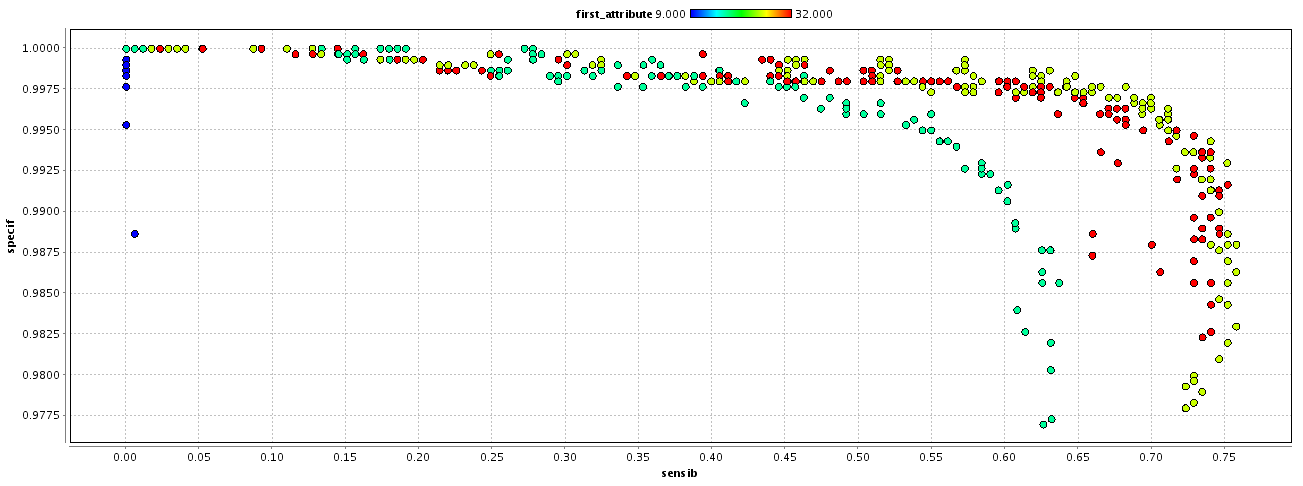
\includegraphics[width=14cm]{images/pareto_param_range}

{\small a) Base Normalisée \'Ecart}

\vspace{0.5cm}

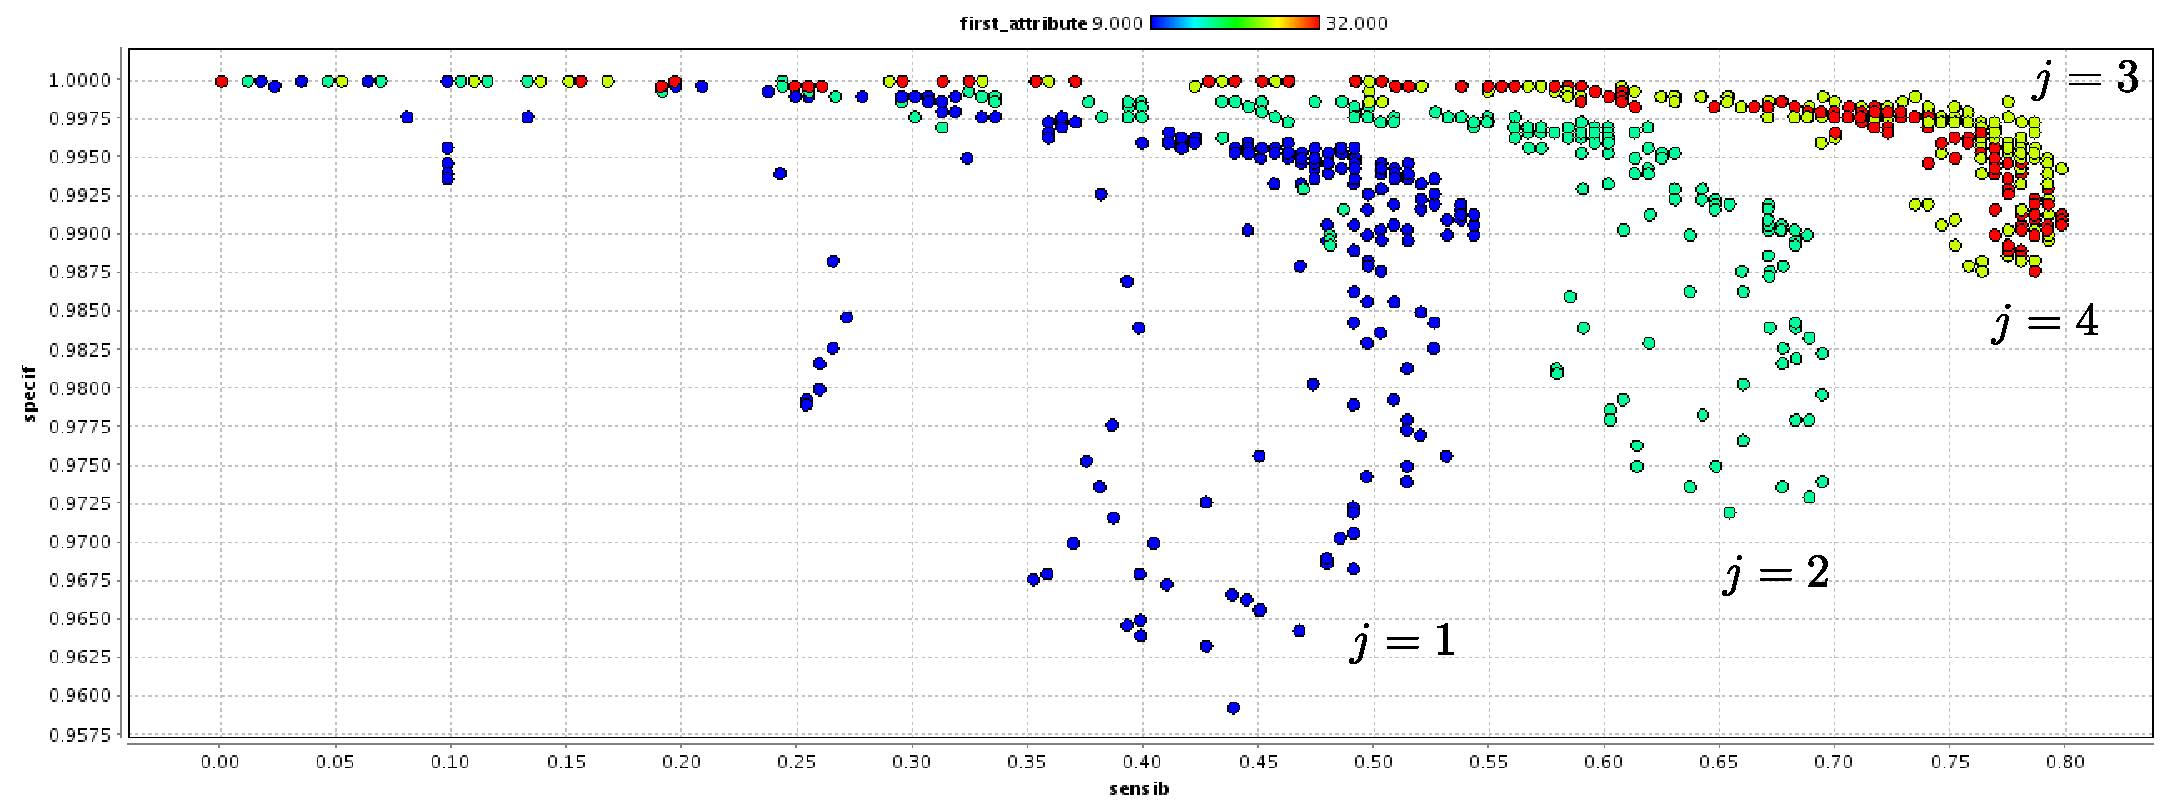
\includegraphics[width=14cm]{images/pareto_param_erosion}

{\small b) Base Érodée}

 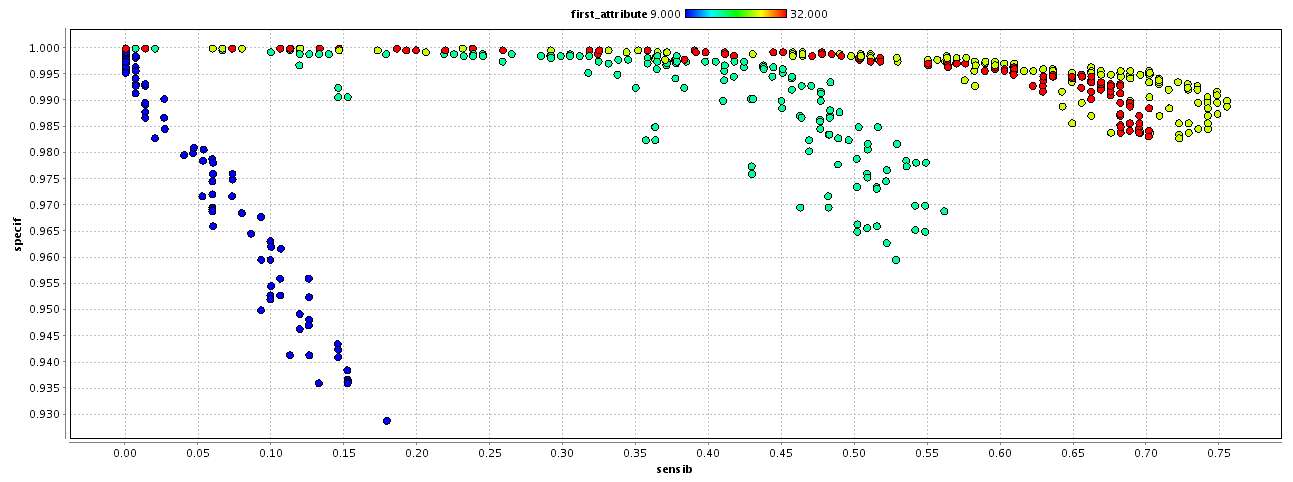
\includegraphics[width=14cm]{images/pareto_param_200_2}

{\small c) Base Témoin 2}

\end{center}
 \caption[(2/2) Recherche des meilleurs paramètres du classifieurs : Fronts de pareto ]{(2/2) Fronts de Pareto des résultats de la recherche des meilleurs paramètres du classifieur. Pour chaque triplet de paramètres $(C, \gamma, j)$, la sensibilité et la spécificité sont reportées sur le graphique. Le code couleur correspond à la valeur de j. En a) la base \textbf{Normalisée Écart} avec 200 points négatifs par image et une normalisation écart. En b), la base \textbf{Érodée}, avec 200 points négatifs par image et une normalisation \emph{moyenne}, en c) la base \textbf{Témoin 2}, réalisée de la même manière que la base \textbf{Témoin} mais en retirant une image. }
\label{fig:paretoParams2}
\end{figure}


Les paramètres du classifieur sont déterminés par une recherche par grille. Elle consiste à rechercher l'optimum en évaluant la performance de chaque jeu de paramètre dans un ensemble déterminé à l'avance. La performance de chaque triplet $(C, \gamma, j)$ est estimée en réalisant une validation croisée à 5 sous-ensembles sur l'ensemble de la base d'apprentissage. 


Les résultats sont reportés sur les figures \ref{fig:paretoParams1} et \ref{fig:paretoParams2} qui tracent, pour chaque base, les variations de spécificité en fonction de la sensibilité pour chaque triplet ($C$, $\gamma$, $j$) évalué sur le poumon. Les paramètres optimaux sont choisis à partir du front de Pareto des figures \ref{fig:paretoParams1} et \ref{fig:paretoParams2} en maximisant la sensibilité.

Dans l'ensemble, on peut voir clairement que les points correspondant au premier niveau de décomposition (bleu foncé) ont une performance systématiquement inférieure aux autres. Pour la base \textbf{Témoin}, la performance maximale est atteinte pour environ 15\% de sensibilité et une spécificité de 93.5\%, ce qui correspond à la valeur de sensibilité la plus faible de tous les points de la base \textbf{Témoin}. On observe cependant un front de Pareto marqué, bien qu'en fort retrait par rapport aux autres niveaux de décomposition. Ce même constat se retrouve pour les bases \textbf{Appauvrie} (1500 points d’apprentissage) et \textbf{Enrichie} (15000 points d’apprentissage). Les trois autres bases montrent des comportements différents. Pour la base \textbf{Normalisée \'Ecart}, les performances pour $j=1$ s'effondrent, de ce fait le classifieur est quasiment incapable de discerner les classes. Cela indique qu'il ne parvient pas à trouver une surface de séparation des données avec les paramètres indiqués. Puisque la normalisation moyenne parvient à mieux séparer les données pour ce niveau de décomposition, il est probable que la normalisation \textbf{\'Ecart} ne parvienne pas à homogénéiser les valeurs des différentes dimensions de manière satisfaisante. Dans le cas de la base \textbf{Érodée}, la simplification du problème de classification fait que les performances sont nettement améliorées : 55\% de sensibilité pour 99.2\% de spécificité, ce qui est le score le plus élevé de toutes les bases. 

Les performances du second niveau de décomposition (bleu ciel) sont toujours situées environ à mi-chemin entre les performances du premier niveau et celles des niveaux 3 et 4.

Les performances des décompositions de niveaux 3 (vert) et 4 (rouge) sont systématiquement meilleures que les deux premières mais sont très variables. La base \textbf{Témoin} et la base \textbf{Appauvrie} montrent une bonne avance tant en terme de sensibilité que de spécificité pour 3 niveaux de décomposition. La base \textbf{Érodée} ne montre, quand à elle, aucune différence de spécificité entre ces deux niveaux de décomposition, mais montre cependant une faible amélioration de la sensibilité pour les 4 niveaux (0.5\%). Quant à la base \emph{Normalisée \'Ecart}, on n'observe pas de réelles différences de performance entre les deux niveaux de décomposition.

La table \ref{fig:paramsParams} référence tous les paramètres sélectionnés à partir des courbes de Pareto. On peut observer que la sensibilité la plus importante est atteinte pour la base \textbf{Appauvrie}, avec 82\% de bonne détection. Ce taux est sensiblement le même que celui de la base \textbf{Érodée} (80\%). Ces valeurs importantes, par rapport aux autres, peuvent s'expliquer par le fait que ces deux bases proposent un problème simplifié. Dans le cas de la base \textbf{Érodée}, les cas litigieux (discontinuités proches des bords des organes) ont été retirés de la base, ce qui simplifie le problème, tandis que pour la base \textbf{Appauvrie}, c'est le nombre de point ''sain`` plus faible (1500 contre 3000) qui permet de rendre le problème plus simple à traiter par le classifieur  au détriment de la généralisation du résultat obtenu.

Il est intéressant de constater que les performances en sensibilité pour les bases \textbf{Appauvrie}, \textbf{Témoin} et \textbf{Enrichie} sont inversement proportionnelles à la taille de la base. En effet, plus la complexité de la base est importante, plus il devient difficile de trouver une surface de séparation efficace. Cependant, une base trop simpliste va engendrer une solution qui sera sans rapport avec la réalité, comme nous le verrons plus loin avec les courbes F-ROC.

Les valeurs de spécificité sont toutes très supérieures à 99\%, ce qui montre que le classifieur n'a pas de problème pour classer correctement les points sains. En effet, la base étant très déséquilibrée, avec un rapport de 17 points sains pour 1 point ''lésion`` dans la base \textbf{Témoin}, il est normal que le classifieur favorise la classification des points ''sain''. Il existe des techniques classiques permettant de compenser ce déséquilibre lors de l'apprentissage, notamment le choix d'un paramètre de pénalisation $C$ différents pour chacune des classes, mais tous les tests que nous avons réalisés n'ont pas montré d'amélioration du résultat. En effet, l'étape de sélection du seuil (voir section suivante) permet de compenser ces différences.

Il est intéressant d'observer que les fronts de Pareto de la base \textbf{Témoin 2} sont très semblables à ceux de la base \textbf{Témoin} pour une décomposition au troisième niveau. Des disparités apparaissent pour le quatrième niveau, mais les performances optimales sont obtenues pour le même jeu de paramètre. Cela semble indiquer que la base d’apprentissage est suffisamment complète en exemples de lésions.
\begin{table}[h!]
\centering
\resizebox{16cm}{!}{
		\begin{tabular}{c c c c c c}
  \hline
   	& Base Témoin 	& Base Érodée	& Base Appauvrie& Base Enrichie & Base Normalisée \\
	&		&		&		&		& Écart \\
  \hline
 C 	& 464		& 74		& 5412		& 5412		& 10000 \\
\hline
$\gamma$& 0.0053	& 0.0094	& 0.00031	& 0.0017	& 0.052 \\
\hline
j	& 3		& 3		& 3		& 4		& 3	\\
\hline
\hline
Sensibilité& 0.75	& 0.80		& \textbf{0.82}		& 0.60		& 0.76	\\
\hline
Spécificité& 0.99	& 0.99		& 0.99		& 0.99		& 0.99 \\
\hline
Précision& 0.98		& 0.98		& 0.97		& 0.99		& 0.98 \\
\hline
 		\end{tabular}
}
\caption[Paramètres $(C,\gamma, j)$ sélectionnés pour l'optimisation des performances sur les différentes bases]{Paramètres $(C,\gamma, j)$ sélectionnés pour l'optimisation des performances sur les différentes bases. Sont indiqués pour chaque base le triplet de paramètres sélectionnés ainsi que sa position sur le front de Pareto.}
\label{fig:paramsParams}
\end{table}

\FloatBarrier

\subsection{Courbe Free-ROC}

Les courbes Free-ROC de la figure \ref{lab:froc_comp_static} permettent de comparer les performances du CAD sur les différentes bases d'apprentissage. Les courbes ont volontairement été tronquées à 40 faux positifs par image, car ce nombre est déjà trop important pour un système CAD.

On peut observer que les courbes correspondants aux bases \textbf{Témoin} et \textbf{Enrichie} atteignent leur maximum de sensibilité pour un nombre de faux positifs relativement faible par rapport aux autres bases : entre 17 et 20 faux positifs pour ces bases, contre plus de 40 pour les bases \textbf{Appauvrie} et \textbf{Érodée}. Cela tend à montrer que le système CAD est plus performant pour ces bases car il crée moins d'agrégats là ou il n'y a pas de lésions.

En ce qui concerne la sensibilité maximale obtenue sur les courbes, elle est atteinte pour la base \textbf{Témoin} avec environ 62\% de sensibilité, suivie par la base \textbf{Appauvrie} avec 60\%, mais pour un nombre de faux positifs beaucoup plus important (38 contre 18 pour la base \textbf{Témoin}). La troisième courbe est la courbe \textbf{Normalisation Écart}, suivie par la base enrichie puis la base \textbf{Érodée}. Il est important de noter que les sensibilités maximales observées sont très proches, entre 55\% et 62\%, ce qui indique que la qualité de la base d'apprentissage n'a pas d'impact réel sur la sensibilité maximale atteinte par le CAD, mais qu'il pourra être plus ou moins difficile pour ce dernier de différencier les lésions du bruit de fond. 

En pratique, on choisira le seuil pour avoir la certitude d'avoir un nombre de faux positifs ``raisonnable'' par image. Dans notre cas, les images contiennent environ 10 lésions par image. Il peut être intéressant de comparer les performances des bases pour un ratio de 1 faux positif par lésion, soit 10 faux positifs. Dans ce cas, la base \textbf{Témoin} a des performances très semblables avec celles de la base \textbf{Enrichie}, à environ 55\%, ce qui est déjà très proche de leurs performances maximales. La base \textbf{Normalisation Écart} et la base \textbf{Appauvrie} sont, quant à elles, à 40\% de sensibilité, tandis que la base \textbf{Érodée} atteint 35\%.


\begin{figure}[h!]
 
 \begin{center}
   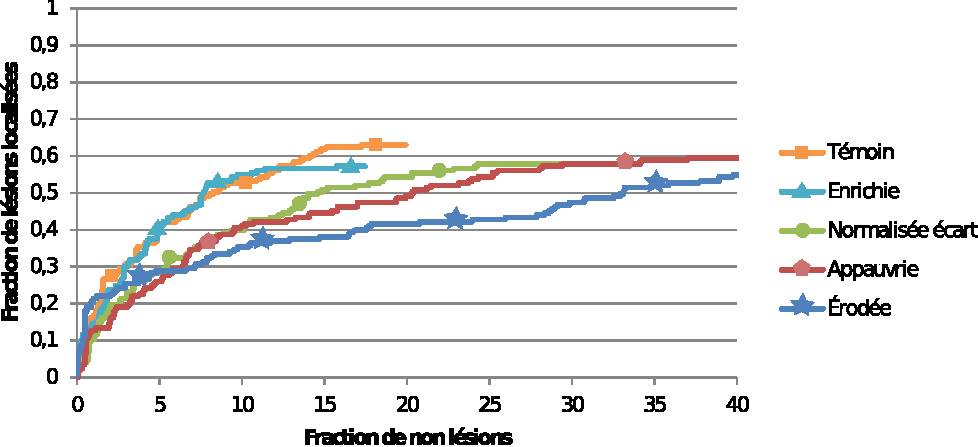
\includegraphics[width=15cm]{images/FROC_param_corrige}
 \end{center}
 \caption[Courbe Free-ROC comparant les performances du CAD selon les différents paramètres de base d'apprentissage]{Courbe Free-ROC comparant les performances du CAD sur une base \textbf{Témoin} (normalisation \emph{moyenne} et 200 points négatifs par image), sur une base \textbf{Enrichie} (1000 points négatifs par image), sur une base \textbf{Appauvrie} (100 points négatifs par image), sur une base \textbf{Normalisée Écart} (normalisation entre -1 et +1 et 200 points négatifs par image) et enfin sur une base de 100 points négatifs par image mais dont les volumes ont été érodés de 2 voxels.}
 \label{lab:froc_comp_static}
\end{figure}


\subsection{Comparaison des performances JAFROC}

La comparaison des performances obtenues par l'algorithme JAFROC \cite{chakraborty1990free} de la figure \ref{lab:fom_param} nous montre les FDM (Figure de Mérite) obtenues pour les différentes bases par l'algorithme JAFROC. Les FDM des bases \textbf{Témoin}, \textbf{Érodée} et \textbf{Enrichie} sont quasiment au même niveau (0.18), mais les barres d'erreurs semblent montrer un léger avantage pour la base \textbf{Témoin}.

Les bases \textbf{Normalisée Écart} et \textbf{Appauvrie} quand à elles ont une FDM de 0.1 environ, ce qui indique une performance plus faible que les autres.

D'un point de vue statistique, la p-valeur (voir \ref{lab:p-valeur}) calculée par le logiciel est de 0.049, ce qui ne permet pas de pouvoir annoncer avec une fiabilité de 95\% que le test est significatif, c'est à dire que les FDM sont effectivement toutes différentes. Cela se vérifie aisément en regardant l'étendue des barres d'erreur. Mais il faut noter que cette FDM est basée sur une méthode avec une puissance statistique faible~\cite{chakraborty2004observer}, ce qui signifie qu'elle sous-estime la p-valeur.

\begin{figure}[h!]
 \begin{center}
   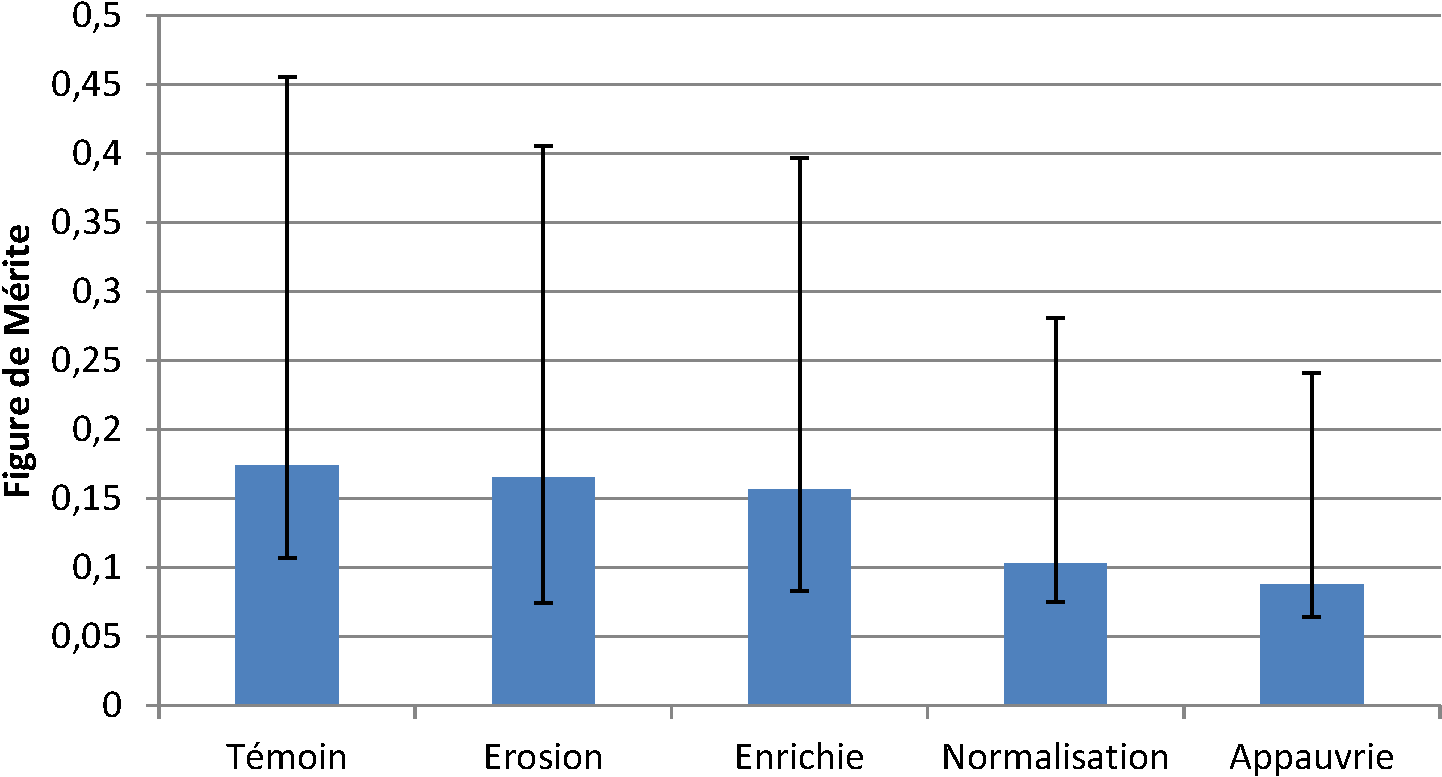
\includegraphics[width=15cm]{images/FOM_param}
 \end{center}
 \caption{Les FDM (Figure de Mérite) JAFROC obtenues pour les différents paramètres de génération de la base d'apprentissage. Les bases Témoin, \'Erodée et Enrichie montrent les meilleures performances, avec un faible avantage pour la base Témoin. Les bases Normélisée écart et Appauvrie ont une figure de mérite nettement plus faible.}
 \label{lab:fom_param}
\end{figure}

\subsection{Conclusion}

Nous avons vu que tous les indicateurs montrent que le maximum de performance est apporté par la base \textbf{Témoin}. De plus, les  performances relativement proches de la base \textbf{Témoin 2} semblent indiquer que les performances sont stables. Nous allons donc conserver les paramètres de cette base pour la comparaison des différents type d'images :

Pas d'érosion, une normalisation visant à ramener la moyenne et l'écart-type sur les caractéristiques à 1, et 200 points extraits de chaque image de la base d'apprentissage.
 

\FloatBarrier

\section{Comparaison des performances de la détection des tumeurs pulmonaires}

Les paramètres de génération de la base d'apprentissage retenus sont ceux de la base \textbf{Témoin}. Ils correspondent aux choix suivants :

\begin{itemize}
 \item 200 points tirés aléatoirement dans le volume complet du poumon de chaque image (hors tumeurs)
 \item normalisation par neutralisation de la moyenne et de la variance, tels que $(\mu, \sigma) = (0,1)$
\end{itemize}


Quatre jeux d'images seront comparés :

\begin{description}
 \item[Statique :] correspond aux images de la ``vérité terrain'', à savoir des images sans mouvement respiratoire. Ce jeu doit donner la performance haute.  
\item[NoCorr :] représente les images simulées avec mouvement respiratoire mais reconstruites sans aucune correction de mouvement. Ce jeu représente le cas le plus défavorable. 
 \item [TE-IM : (Transformation Elastique images) :] correspond aux images reconstruites avec la correction de mouvement post-reconstruction.
 \item [TE-MS (Transformation Elastique Matrice Système) :] correspond aux images reconstruites avec correction de mouvement pendant la reconstruction.
\end{description}


\begin{figure}[h!]

\begin{center}
 
\includegraphics[width=14cm]{images/pareto_mod_IM}

{\small a) TE-IM}
\vspace{0.5cm}

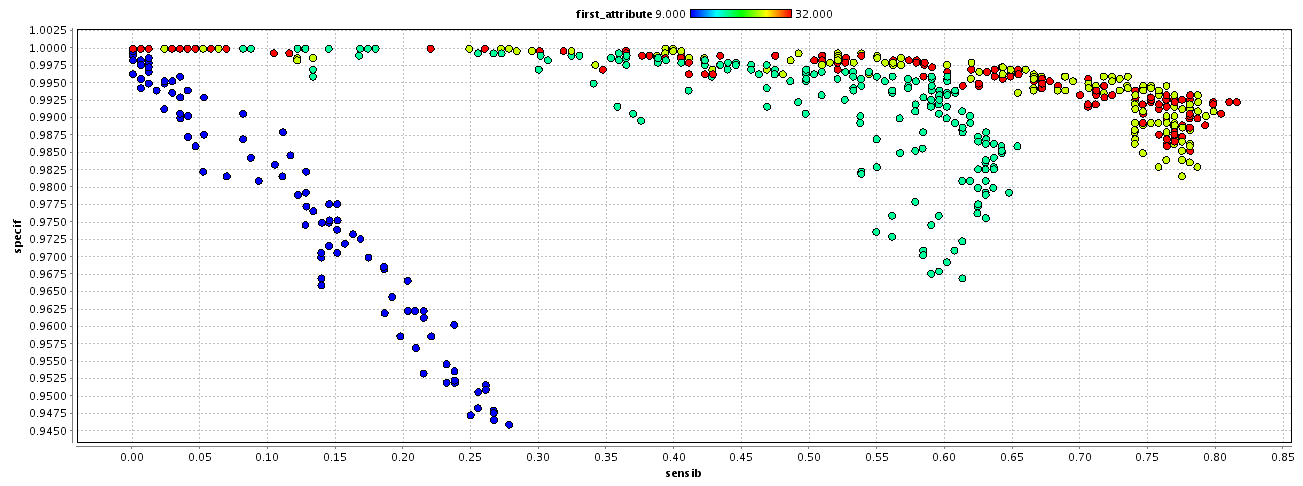
\includegraphics[width=14cm]{images/pareto_mod_LOR}
 
{\small b) TE-MS}
\vspace{0.5cm}


\includegraphics[width=14cm]{images/pareto_mod_NoCorr}

{\small c) NoCorr}

\end{center}
 \caption[Fronts de Pareto des résultats de la recherche des meilleurs paramètres du classifieur pour les différents jeux d'images pulmonaire]{Fronts de Pareto des résultats de la recherche des meilleurs paramètres du classifieur pour les différents jeux d'images pulmonaire, avec 200 points négatifs par image. Pour chaque triplet de paramètres $(C, \gamma, j)$, la sensibilité et la spécificité sont reportées sur le graphique. Le code couleur correspond à la valeur de j. a) représente la correction d'image \textbf{TE-IM}, b) les images non corrigées du mouvement, et c) les images corrigées par la méthode LOR.}
\label{fig:paretoModalite} 
\end{figure}








\begin{table}[h!]
	\begin{center}
		\begin{tabular}{c| c c c c c}
  \hline
  a	& Base Statique	& Base TE-IM	& Base TE-MS	& Base NoCorr	\\
  \hline
 C 	& 464		& 10000		& 10000		& 10000		\\
\hline
$\gamma$& 0.0053	& 0.00097	& 0.00031	& 0.00055	\\
\hline
j	& 3		& 3		& 4		& 3		\\
\hline
\hline
Sensibilité& 0.75	& 0.81		& 0.82		& 0.83	\\
\hline
Spécificité& 0.99	& 0.99		& 0.99		& 0.99		\\
\hline
Précision& 0.98		& 0.98		& 0.98		& 0.98		\\
\hline
 		\end{tabular}

	\end{center}
\caption[Paramètres sélectionnés pour l'optimisation des performances de détection des tumeurs pulmonaires]{Paramètres sélectionnés pour l'optimisation des performances de détection des tumeurs pulmonaires. Chaque triplet de paramètres sélectionné $(C,\gamma,j)$ est indiqué ainsi que sa valeur se sensibilité et spécificité.}
\label{tab:paramsModPoumon}
\end{table}

\subsection{Sélection des meilleurs paramètres du classifieur}

De la même manière que pour la sélection de la meilleure base d'apprentissage, il faut adapter les paramètres du classifieur ($C$, $\gamma$, $j$) aux bases des quatre jeux d'images que nous souhaitons comparer.

La figure \ref{fig:paretoModalite} montre les nuages de points associés aux différents triplets de paramètres ($C$, $\gamma$, $j$) pour chaque type d'images. Les performances des images statiques sont celles présentées sur la base \textbf{Témoin} de la figure \ref{fig:paretoParams1}.a. La table \ref{tab:paramsModPoumon} résume les triplets ($C$, $\gamma$, $j$) correspondant aux meilleures performances mesurées à l'aides des nuages de points des figures \ref{fig:paretoParams1}.a et \ref{fig:paretoModalite}.

Il est étonnant de constater que la base \ref{fig:paretoParams1}.a, qui correspond aux images \textbf{Statique}, offre les plus mauvaises performances pour la décomposition de niveau 1 (17\% de sensibilité). La mauvaise performance de cette base d'apprentissage se retrouve pour tous les niveaux de décomposition. Le résultat est également souligné par le tableau \ref{tab:paramsModPoumon} (sensibilité de 75\% contre des valeurs supérieures à 80\% pour les autres type d'images). On peut cependant observer que les nuages de points des autres jeux d'images ont la même distribution spatiale que ceux de la base \textbf{Statique}, par opposition aux distributions des bases \textbf{Érodée} ou \textbf{Normalisée Écart} vues dans la partie précédente. Par exemple, pour $j=1$, on observe une forte corrélation de la sensibilité et de la spécificité pour les base \textbf{Statique}, \textbf{NoCorr}, \textbf{TE-IM} et \textbf{TE-MS} que l'on ne retrouve pas pour les bases \textbf{Érodée} et \textbf{Normalisée Écart}. 

On peut observer qu'il y a une forte corrélation entre la sensibilité et la spécificité des points pour tous les types d'images au premier niveau de décomposition.

Le type d'images ayant les meilleures performances pour la décomposition de niveau 2 est \textbf{TE-IM}, avec plus de 70\% de sensibilité, comparés aux 60\% de la base \textbf{Statique}. 

Les meilleures performances du CAD sont atteintes pour le troisième niveau de décomposition pour tous les types d'images sauf \textbf{TE-MS}, avec une sensibilité d'environ 81 et 83\% pour TE-IM et NoCorr, et 75\% pour la base \textbf{Statique}. Les performances maximales sur TE-MS sont atteintes pour $j=4$.

La spécificité observée pour les meilleurs jeux de paramètres est sensiblement la même quelque soit le type d'image, entre 99\% et 99.5\%.

\subsection{Courbes Free-ROC}

Les courbes F-ROC obtenues sur les différents type d'images à l'aide des triplets ($C$, $\gamma$, $j$) reportés dans la table~\ref{tab:paramsModPoumon} sont présentées dans la figure \ref{fig:froc_mod}. 

Toutes les courbes ont un NFM (nombre de faux positifs moyen par image) à la sensibilité maximale à peu près équivalent entre 20 et 24, excepté TE-MS avec un NFM à la sensibilité maximale de 34. Cependant, les performances en FLL (fraction  des lésions détectées et localisées) de TE-MS sont constantes à partir d'une NFM de 20 environ. 

L'ordre des courbes est constant pour tous les NFM à partir de 5 faux positifs par image. Au delà de cette limite, les performances des images \textbf{statique} sont supérieures à celles de \textbf{TE-IM} de 1 à 5\%, tandis que \textbf{TE-IM} a des performances supérieures de 3 à 10\% à celles des images \textbf{TE-MS} et des images \textbf{NoCorr}. Ces deux dernières ont des performances quasiment identiques.

En dessous de 5 faux positifs par image, les courbes sont trop proches pour pouvoir en déduire une tendance.


Globalement, le graphique montre que le maximum de performance est apporté par la base \textbf{Statique}, suivi par la base \textbf{TE-IM}. Les bases \textbf{TE-MS} et \textbf{NoCorr} sont très proches l'une de l'autre mais nettement en dessous des deux premières en terme de FLL, à NFM égale.

%\todo{vérifier plus de FLN}
\begin{figure}[h!]
 \begin{center}
   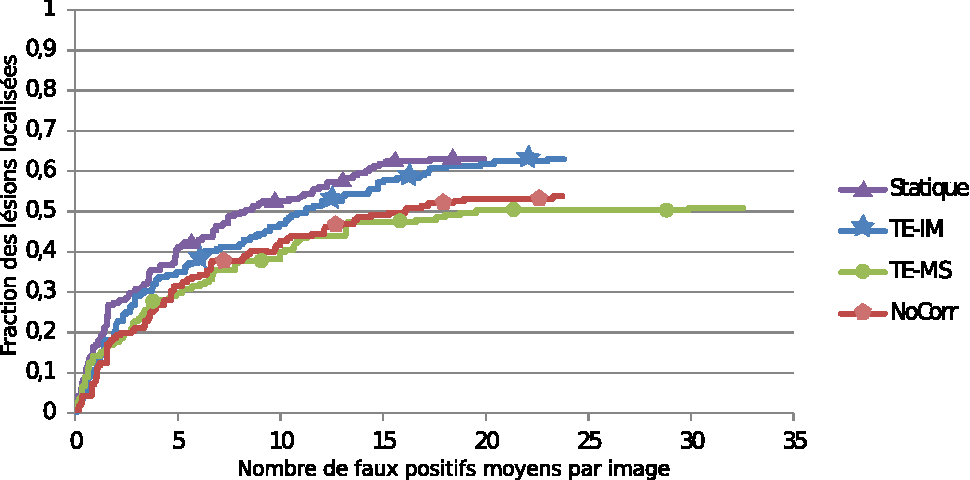
\includegraphics[width=13cm]{images/FROC_mod_corrige}
 \end{center}
 \caption{Courbe Free-ROC comparant les performances du CAD selon la technique de correction du mouvement respiratoire.}
 \label{fig:froc_mod}
\end{figure}


\subsection{Comparaison des performances JAFROC}

Les figures de mérite obtenues par l'algorithme de JAFROC sont présentées dans la figure \ref{fig:fom_mod}. On observe une tendance proche de celle observée sur les courbes F-ROC. Les images \textbf{Statique} montrent les meilleures performances, suivies par \textbf{TE-IM}. Il est intéressant de noter que les valeurs de \textbf{TE-IM} et \textbf{TE-MS} sont relativement proches, y compris leurs mesures d'erreur, ce qui indique que l'algorithme JAFROC les distingue difficilement. \textbf{TE-MS} est quand à lui nettement en retrait. 

\begin{figure}[h!]
 \begin{center}
   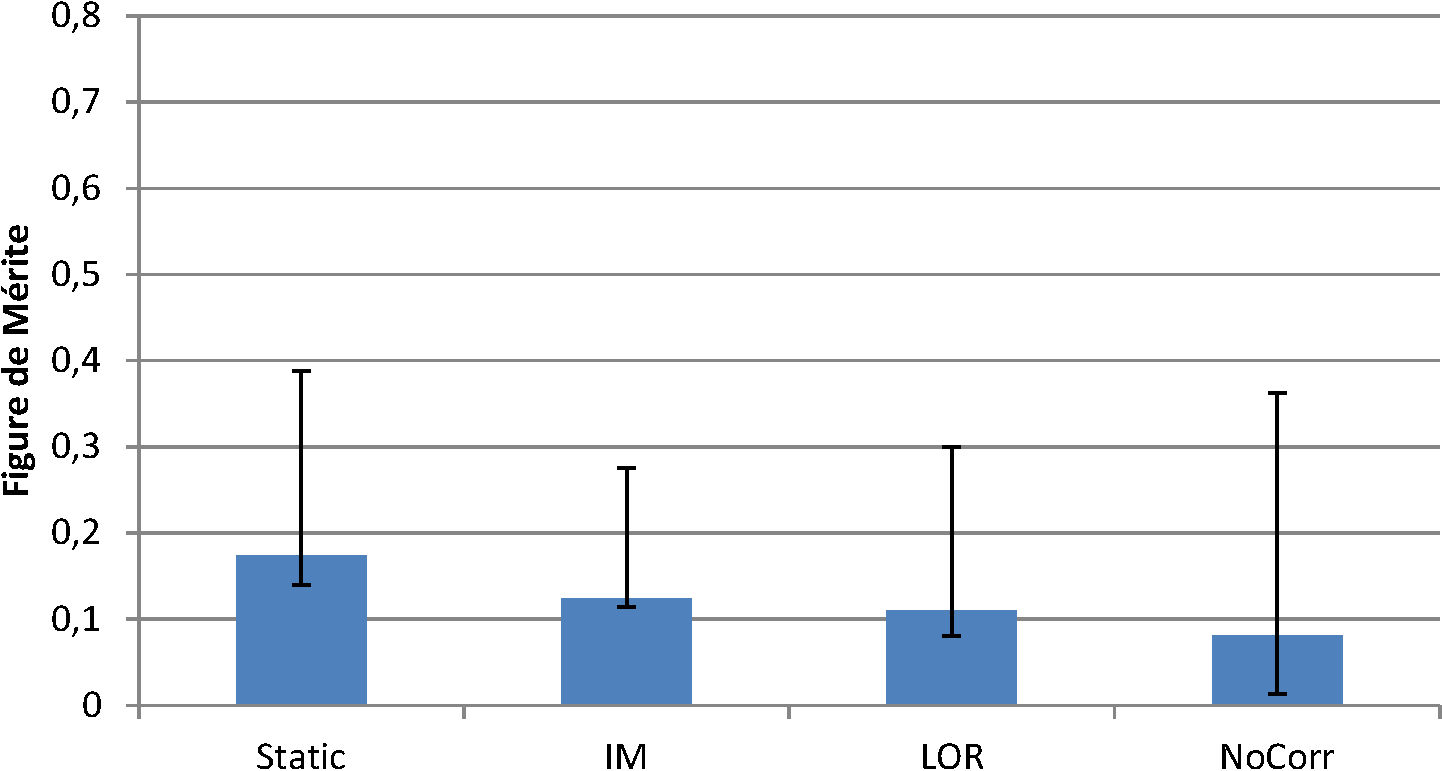
\includegraphics[width=13cm]{images/FOM_mod}
 \end{center}
 \caption{Les FDM (Figure de Mérite) obtenues pour les différentes techniques de correction du mouvement respiratoire sur la détectabilité des lésions du poumon.}
 \label{fig:fom_mod}
\end{figure}

\subsection{Conclusion}

Les résultats présentés précédemment indiquent que les techniques de correction du mouvement respiratoire améliorent les performances de détection par rapport aux images non corrigées pour les lésions pulmonaires. Le résultat est net pour \textbf{TE-IM}, surtout lorsque l'on regarde les courbes F-ROC. Il est plus difficile de statuer sur les performances de la méthode \textbf{TE-MS}, dont les performances selon JAFROC sont au même niveau que celles de la méthode \textbf{TE-IM}, mais qui est nettement moins performante que cette dernière sur les courbes F-ROC.


\FloatBarrier

\section{Comparaison des performances des différentes méthodes pour la détection des tumeurs hépatiques}


\subsection{Sélection des meilleurs paramètres du classifieur}

Les figures \ref{fig:paretoModalite19_1} et \ref{fig:paretoModalite19_2} nous montrent une répartition des performances très différente de celle observée précédemment pour les travaux sur les tumeurs pulmonaires. 

Pour le premier niveau de décomposition ($j=1$), les images \textbf{Statique}, \textbf{TE-IM} et \textbf{TE-MS} montrent une très grande dispersion des valeurs de performances. \textbf{NoCorr}, par contre, montre des points plus proches, mais avec des sensibilités très faibles (inférieures à 15\%). Cette dispersion montre une rupture par rapport à la corrélation observée sur les bases du poumon.

De la même manière que pour $j=1$, les performances obtenues pour $j=2$ montrent une dispersion très importante des points pour les images \textbf{Statique} et \textbf{TE-IM}. Le nuage de points correspondant à \textbf{TE-MS} a une forme plus proche de celles observées précédemment. La base non corrigée est clairement en difficulté car l'apport des informations du second niveau de décomposition diminue les performances maximales du CAD en sensibilité.

En ajoutant les informations des niveaux de décomposition supérieurs, on observe une amélioration nette des performances, surtout pour la base \textbf{NoCorr}. Tous les type d'images montrent une amélioration des performances lorsque l'on  prend en compte le 4è niveau de décomposition, par opposition aux tumeurs du poumon où l'ajout de ces informations faisait baisser les performances du CAD. \'Etant donné que les informations fournies par le quatrième niveau de décomposition des ondelettes sont de très basse fréquence, elles ne donnent pas d'information sur la lésion elle-même mais sur son environnement. Cela semble indiquer que le classifieur est mal adapté pour gérer ces données.


Les résultats des couples ($C$, $\gamma$, $j$) pour les quatre types d'images sont reportés dans le tableau \ref{fig:paramsModFoie}. Comme pour les lésions pulmonaires, \textbf{TE-IM} a la sensibilité la plus forte avec 68\%. Et cette fois ci, \textbf{Statique} est seconde avec 62\%.

\begin{figure}[h!]

\begin{center}
 
\includegraphics[width=14cm]{images/pareto_mod_Static19}

{\small a) Statique}
\vspace{0.5cm}

 
\includegraphics[width=14cm]{images/pareto_mod_IM19}

{\small b) TE-IM}

\end{center}
 \caption[(1/2) Fronts de Pareto des résultats de la recherche des meilleurs paramètres du classifieur pour les lésions du foie]{Fronts de Pareto des résultats de la recherche des meilleurs paramètres du classifieur pour les lésions du foie, avec 200 points négatifs par image. Pour chaque triplet de paramètres (C, $\gamma$, j), la sensibilité et la spécificité sont reportées sur le graphique. Le code couleur correspond à la valeur de j. a) représente les images statiques, b) les images corrigées du mouvement post-reconstruction.}
\label{fig:paretoModalite19_1}
\end{figure}

\begin{figure}[h!]

\begin{center}
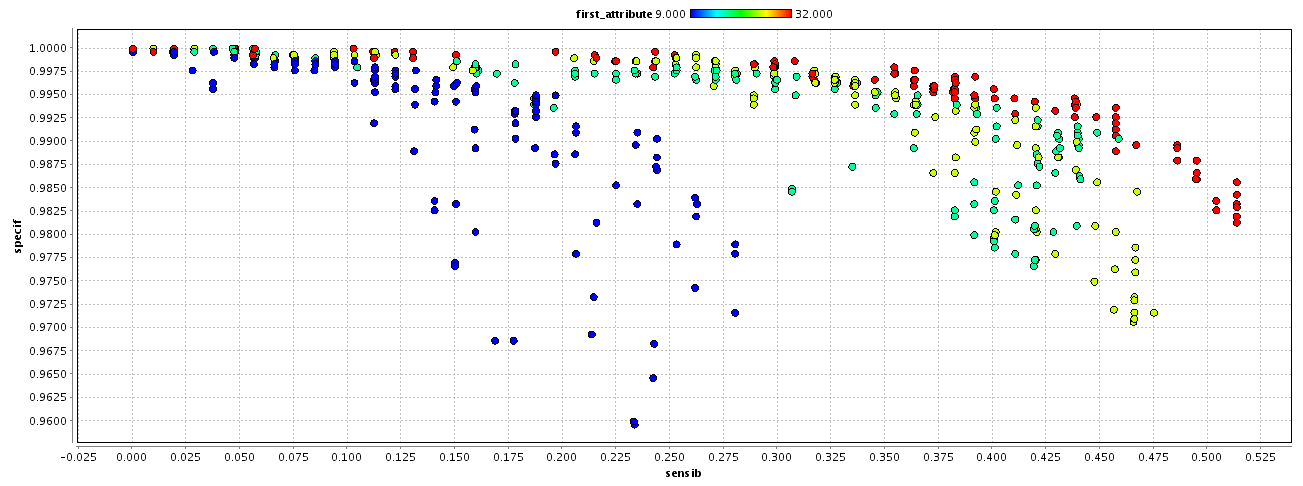
\includegraphics[width=14cm]{images/pareto_mod_LOR19}
 
{\small c) TE-MS}
\vspace{0.5cm}


\includegraphics[width=14cm]{images/pareto_mod_NoCorr19}

{\small d) NoCorr}

\end{center}
 \caption[(2/2) Fronts de Pareto des résultats de la recherche des meilleurs paramètres du classifieur pour les lésions du foie]{Fronts de Pareto des résultats de la recherche des meilleurs paramètres du classifieur pour les lésions du foie, avec 200 points négatifs par image. Pour chaque triplet de paramètres $(C, \gamma, j)$, la sensibilité et la spécificité sont reportées sur le graphique. Le code couleur correspond à la valeur de j. c) représente la correction d'image pendant la reconstruction et d) le images non corrigées.}
\label{fig:paretoModalite19_2} 
\end{figure}

% Static : 857.6958985908936	0.001709975946676697	32.0	0.9790779315594078	0.6160173160173159	0.992
% LOR	 : 251.18864315095797	0.005323362023203629	32.0	0.969422309209811	0.5134199134199134	0.9856666666666667 
% NoCorr : 5411.6952654646375	0.001709975946676697	32.0	0.9417478291936561	0.30779220779220784	0.9643333333333333
% IM	 : 5411.6952654646375	5.49280271653059E-4	32.0	0.9826195691007659	0.6805194805194804	0.9933333333333334
\begin{table}[h!]
\begin{center}
		\begin{tabular}{c| c c c c c}
  \hline
  a	& Base Statique	& Base TE-IM	& Base TE-MS	& Base NoCorr	\\
  \hline
 C 	& 858		& 5412		& 251		& 5412		\\
\hline
$\gamma$& 0.002		& 0.00055	& 0.0053	& 0.0017	\\
\hline
j	& 4		& 4		& 4		& 4		\\
\hline
\hline
Sensibilité& 0.62	& 0.68		& 0.51		& 0.31	\\
\hline
Spécificité& 0.99	& 0.99		& 0.99		& 0.96		\\
\hline
Précision& 0.98		& 0.98		& 0.97		& 0.94		\\
\hline
 		\end{tabular}

\end{center}
\caption[Paramètres sélectionnés pour l'optimisation des performances du CAD sur les tumeurs hépatiques]{Paramètres sélectionnés pour l'optimisation des performances du CAD sur les tumeurs hépatiques. Sont indiqués pour chaque base le triplet de paramètres sélectionné ainsi que sa position sur le front de Pareto.}
\label{fig:paramsModFoie}
\end{table}

\subsection{Courbes Free-ROC}

\begin{figure}[h!]
 \begin{center}
   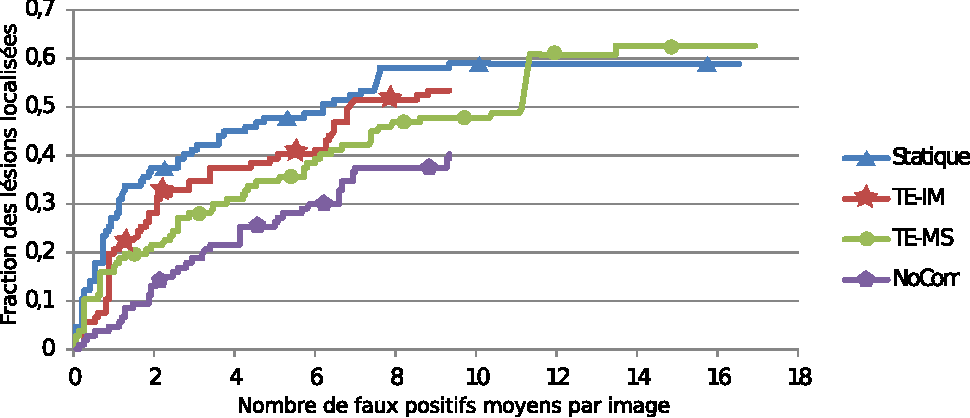
\includegraphics[width=15cm]{images/FROC_mod19_corrige}
   \vspace{-0.3cm}
 \end{center}
 \caption{Courbe Free-ROC comparant les performances du CAD selon les techniques de correction du mouvement respiratoire.}
\label{fig:froc_mod19}
\end{figure}


Les courbes Free-ROC de la figure \ref{fig:froc_mod19} montrent un ordre différent de celui présenté par l'analyse JAFROC de la figure~\ref{fig:fom_mod19}.

Le maximum de performances est apporté par les images statiques, suivi par les images \textbf{TE-IM}, puis \textbf{TE-MS} et enfin \textbf{NoCorr}. Contrairement au poumon, les courbes sont relativement bien séparées avec une différence de sensibilité de 20\% entre les images non \textbf{NoCorr} et \textbf{Statique}. 

Il est étonnant d'observer que les images \textbf{Static} et \textbf{TE-MS} ont toutes les deux un NFM maximum d'environ 17, très supérieur à celui de \textbf{TE-IM} et des images non corrigées qui ne dépassent pas 9 faux positifs par image. Mais comme dans les cas précédents, ce nombre important de faux positifs n'apporte qu'une amélioration très faible de la sensibilité pour les images de la base \textbf{Statique}, au contraire de \textbf{TE-MS} où un important bond de sensibilité (de 50\% à 60\%) apparaît pour un NFM de 11.5 . 

Si l'on se contente de comparer les courbes F-ROC pour un NFM donné de 9, la base d'images \textbf{Statique} a la meilleur sensibilité avec 58\%, suivie par \textbf{TE-IM} avec 53\% et \textbf{TE-MS} avec 48\%. Les images \textbf{NoCorr} sont en net retrait avec seulement 37\% de sensibilité.

Les performances sont globalement en retrait par rapport à celles du poumon, mais l'ordre des courbes reste cohérent avec celui observé sur le poumon.


\subsection{Comparaison des performances JAFROC}

\begin{figure}[h!]
 \begin{center}
   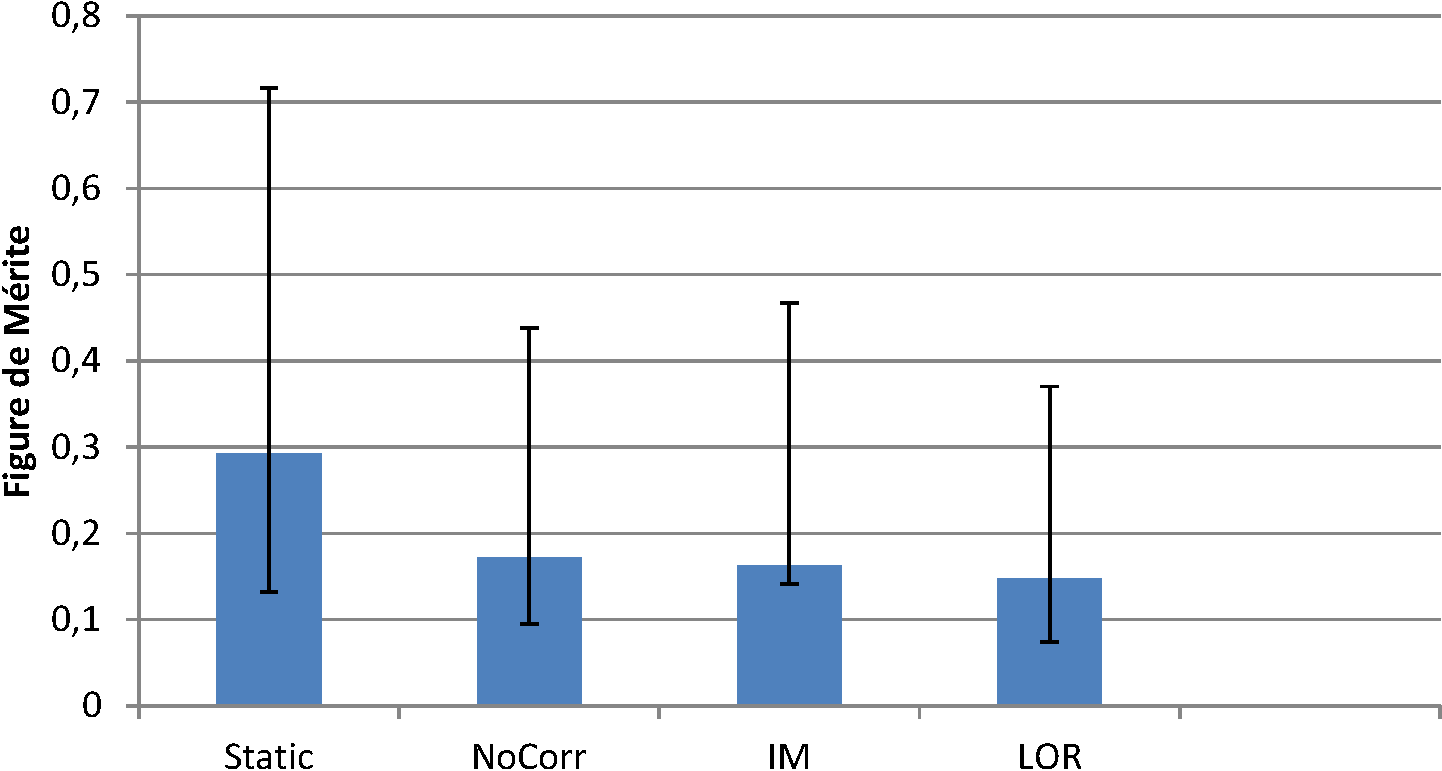
\includegraphics[width=15cm]{images/FOM_mod19}
 \end{center}
 \caption{Les FDM (Figure de Mérite) JAFROC obtenues pour les différents type d'images pour la détectabilité des lésions du foie.}
 \label{fig:fom_mod19} 
\end{figure}


Les Figures de mérite obtenues par l'algorithme de JAFROC sont présentées dans la figure \ref{fig:fom_mod19}. La p-valeur est de 0.1, ce qui ne permet pas de déclarer que statistiquement les données sont différentes.
Il n'est pas étonnant de constater que les FDM sont plus élevées que précédemment car le nombre de faux positifs est pratiquement deux fois inférieur à celui obtenu pour le poumon, ce qui est le signe que le classifieur réussit mieux à discerner les vrais positifs.

On observe que les images \textbf{statique} ont un score supérieur de 60\% environ à celui des images \textbf{NoCorr}. Par contre, il est surprenant de constater que les deux techniques de correction du mouvement respiratoire ont un score égal ou plus faible que les images non corrigées, en contradiction avec les résultats de l'analyse F-ROC. Cependant, la proximité des valeurs ne permet pas de montrer une réelle hiérarchie entre les jeux d'images. Tout au plus pourrait-on observer que l'étendue des barres d'erreur semble indiquer que \textbf{TE-IM} aurait de meilleures performances que les images \textbf{NoCorr}, elles-mêmes supérieures aux images \textbf{TE-MS}, mais il est n'est pas possible de se prononcer de manière définitive à partir de ces données. 




\subsection{Conclusion}

Les résultats des mesures de performance sur les tumeurs hépatiques sont contrastés. Les courbes F-ROC montrent un clair avantage des techniques de correction du mouvement respiratoire, surtout pour \textbf{TE-IM} si l'on compare la sensibilité pour un nombre moyen de fausses localisations. Par contre, les figures de mérite obtenues par JAFROC montrent à l'inverse que \textbf{TE-IM} et \textbf{TE-MS} sont au même niveau que les images non corrigées du mouvement, en net retrait par rapport aux images \textbf{Statique}.





